\documentclass[arial,pdftex]{beamer}
\usepackage{graphicx}
\usepackage{pgfplots}

\pgfplotsset{compat=1.3}


\title{The Beauty of Plone}
\subtitle{a beautiful CMS}

\author{Chris Perivolaropoulos}

% \AtBeginSection[]{\begin{frame}\frametitle{Table of Contents}\tableofcontents[currentsection]\end{frame}}

\begin{document}
\section{Who am I}
\frame{\titlepage}

\section{What is a CMS}

\subsection{History}
\begin{frame}{In the beginning there was HTML}
  \begin{center}
    
\includegraphics[width=0.5\textwidth]{html.pdf}
  \end{center}
\end{frame}

% a slide with a picture i drew with html files

% say that they were many, repetitive, hard to maintain
% Show different things to each user: dynamic pages
%
% users

\begin{frame}{Then there were scripts}
  \begin{center}
    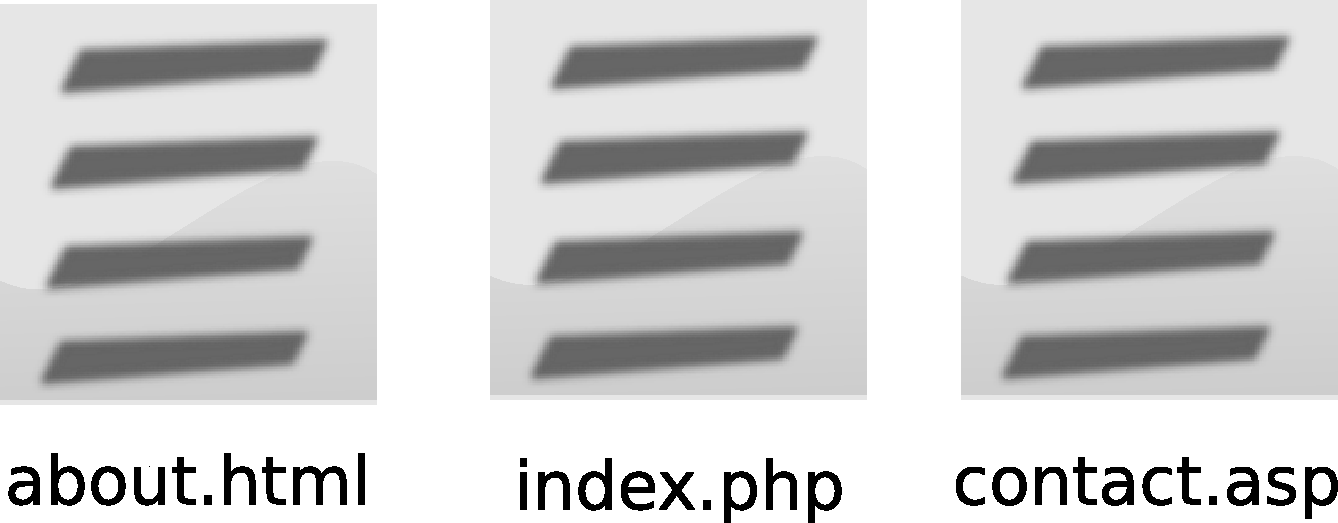
\includegraphics[width=0.5\textwidth]{scripts.pdf}
  \end{center}
\end{frame}

% a slide with a picture of php asp and html
%
% how nice things were
% scripts were many, only technical people could manage, again
% repetitive among developers

\frame{CMSs were born}

% scripts were unified in a single program
% the developers have less work to do and focus in taking things further
% the designers dont have to worry about programming
% editors can focus on writing

\subsection{Today}
% the job of a cms
\frame{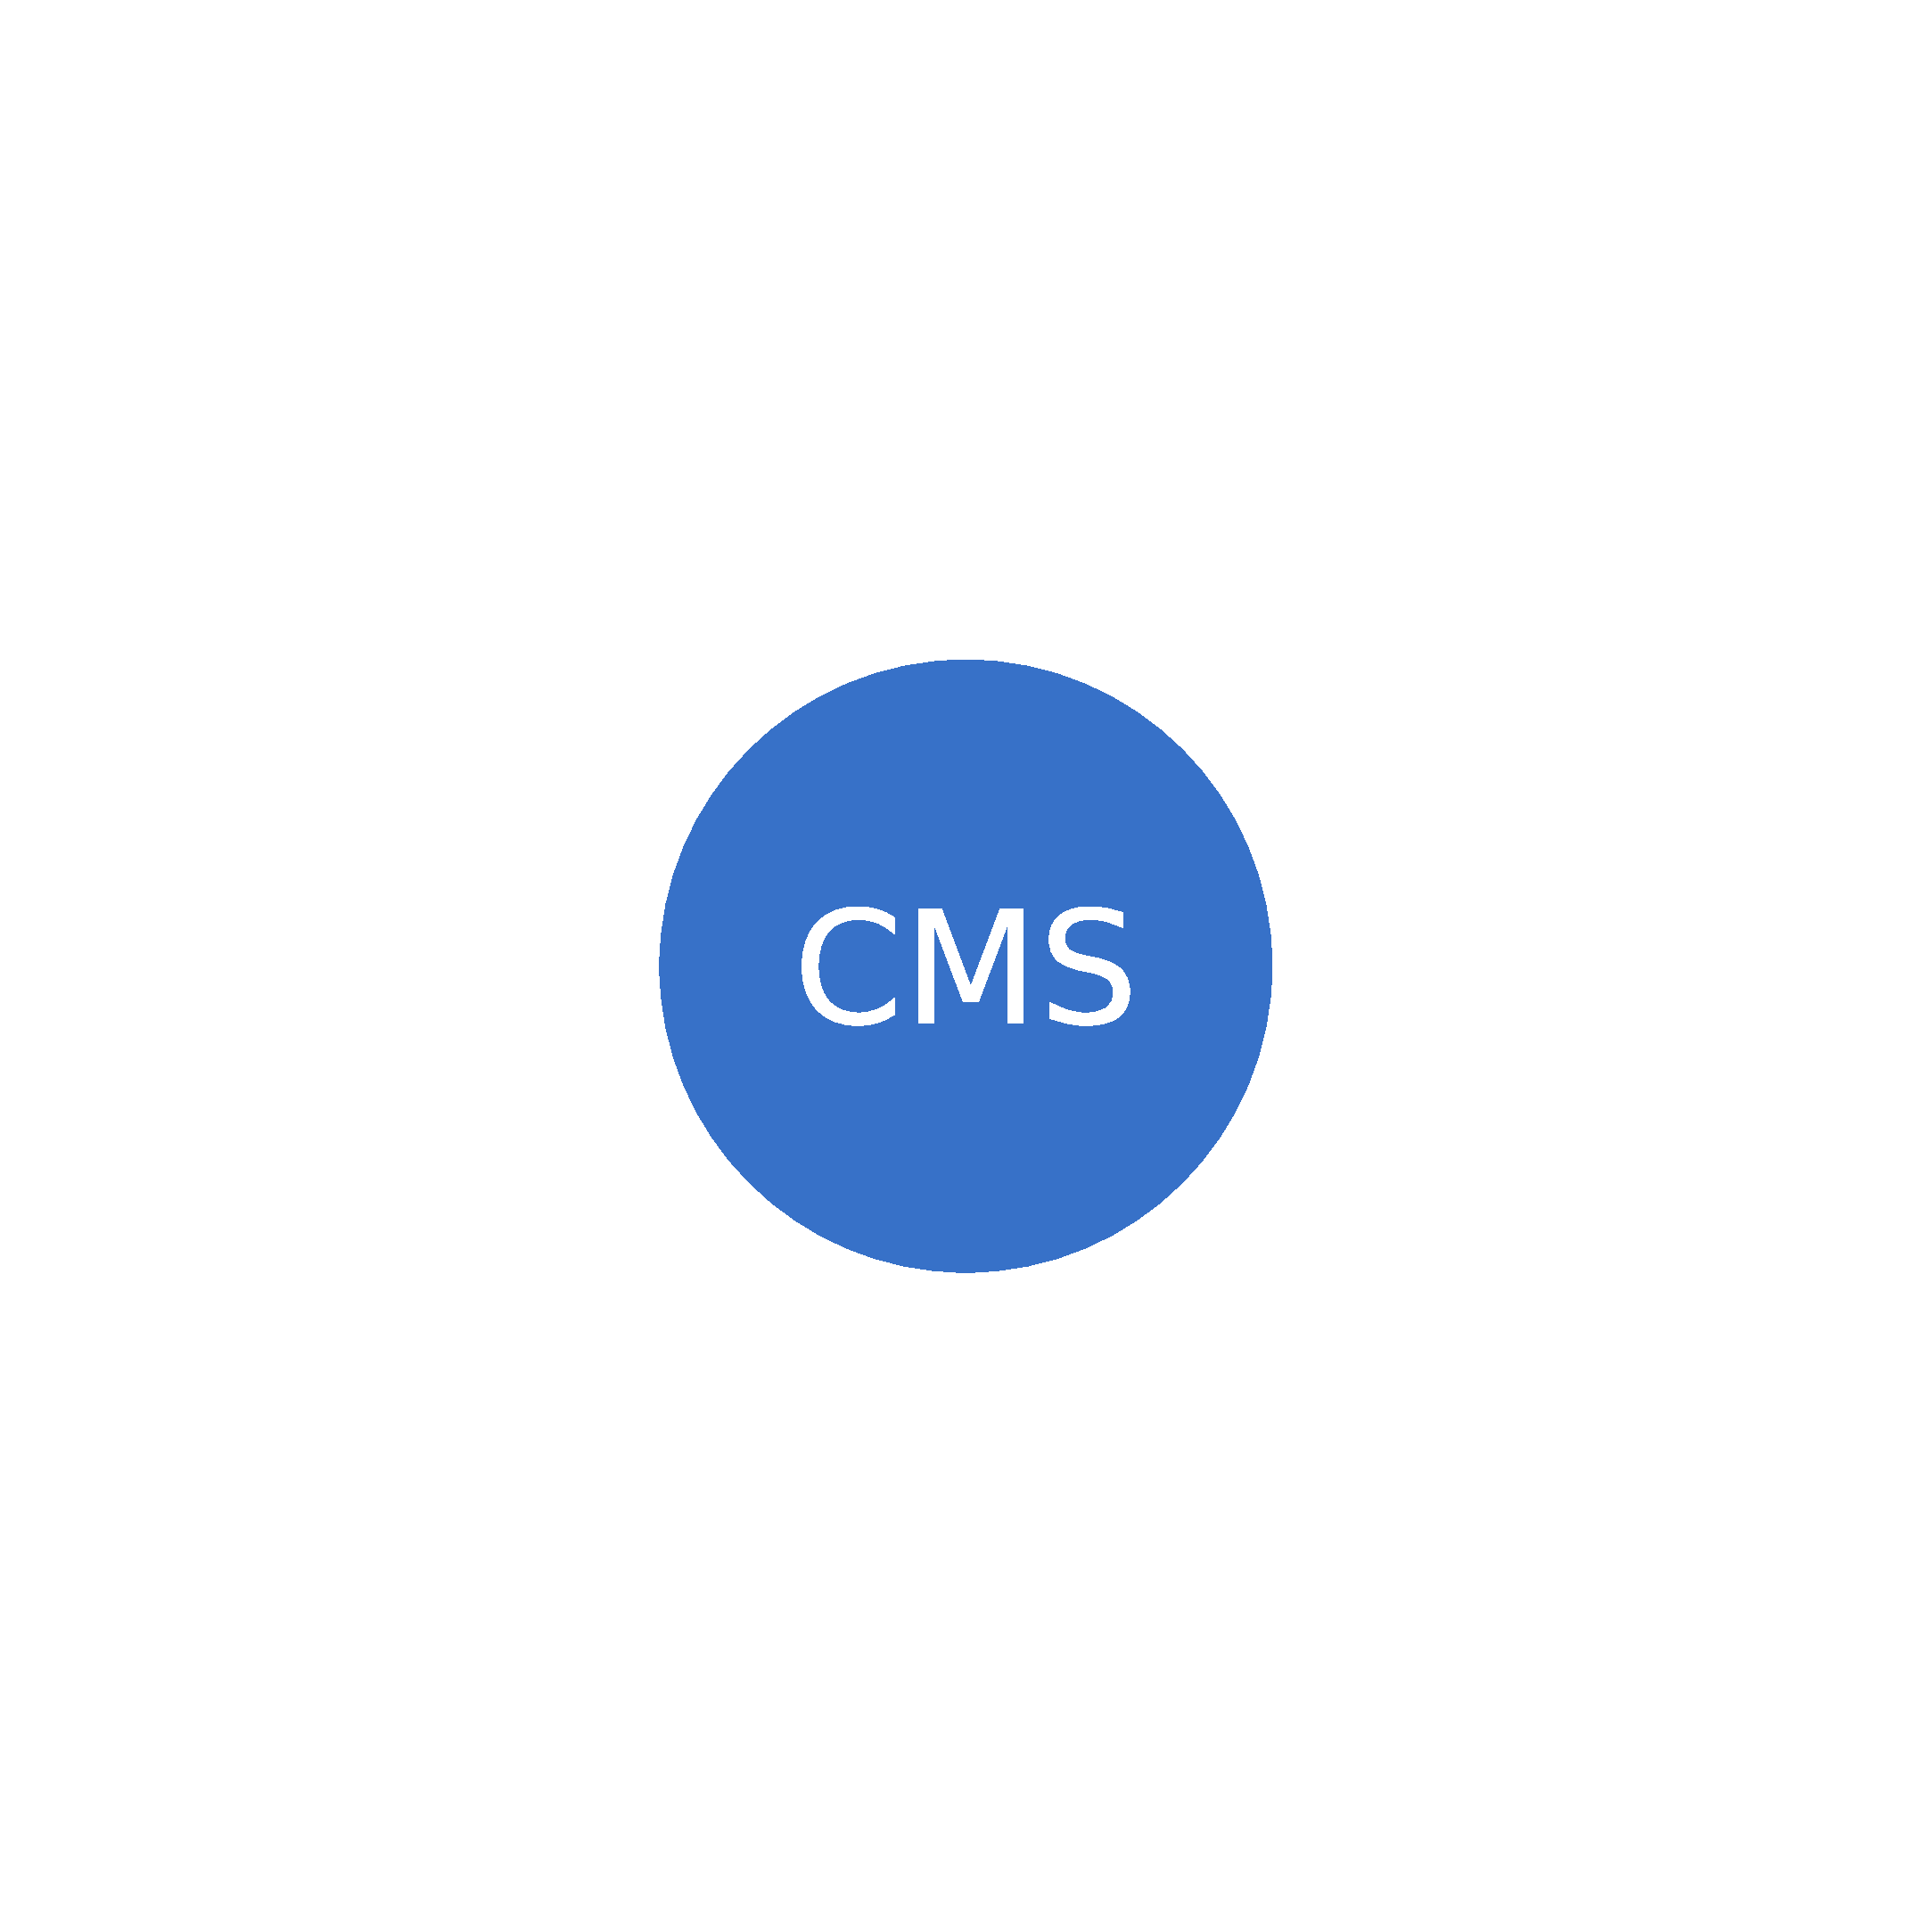
\includegraphics[height=\textheight]{cms.pdf}}
\frame{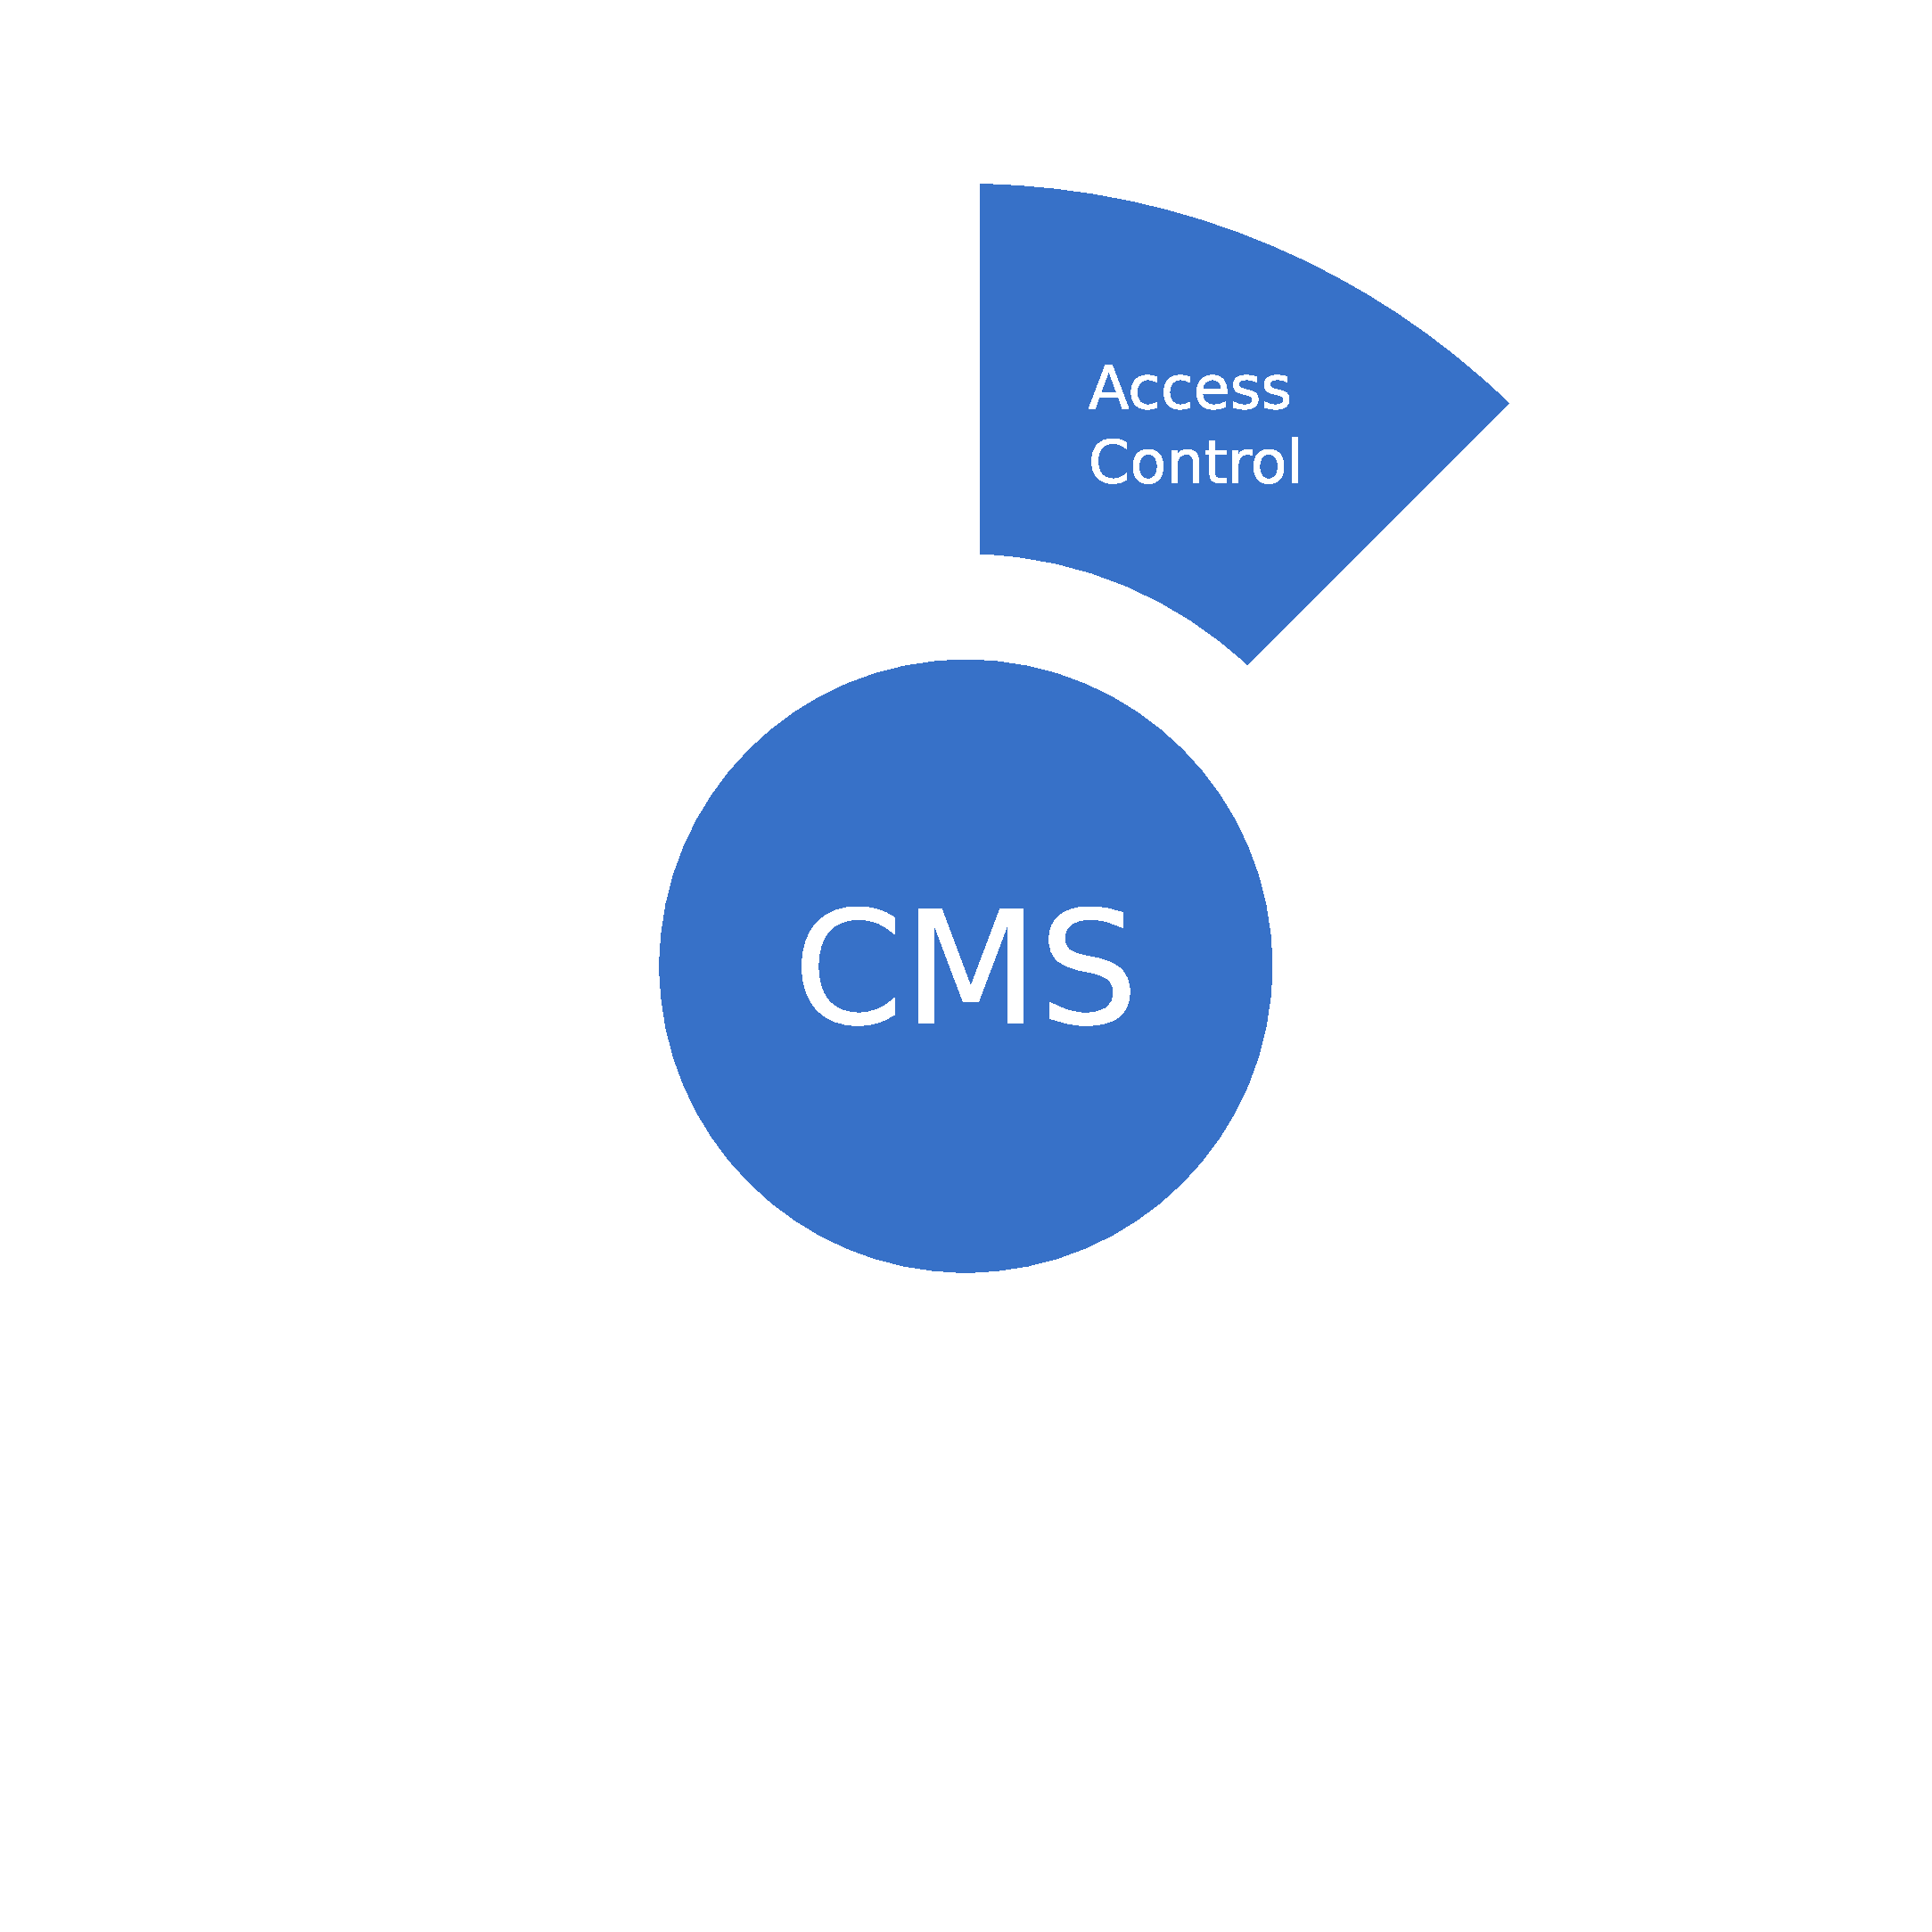
\includegraphics[height=\textheight]{cms-access-control.pdf}}
\frame{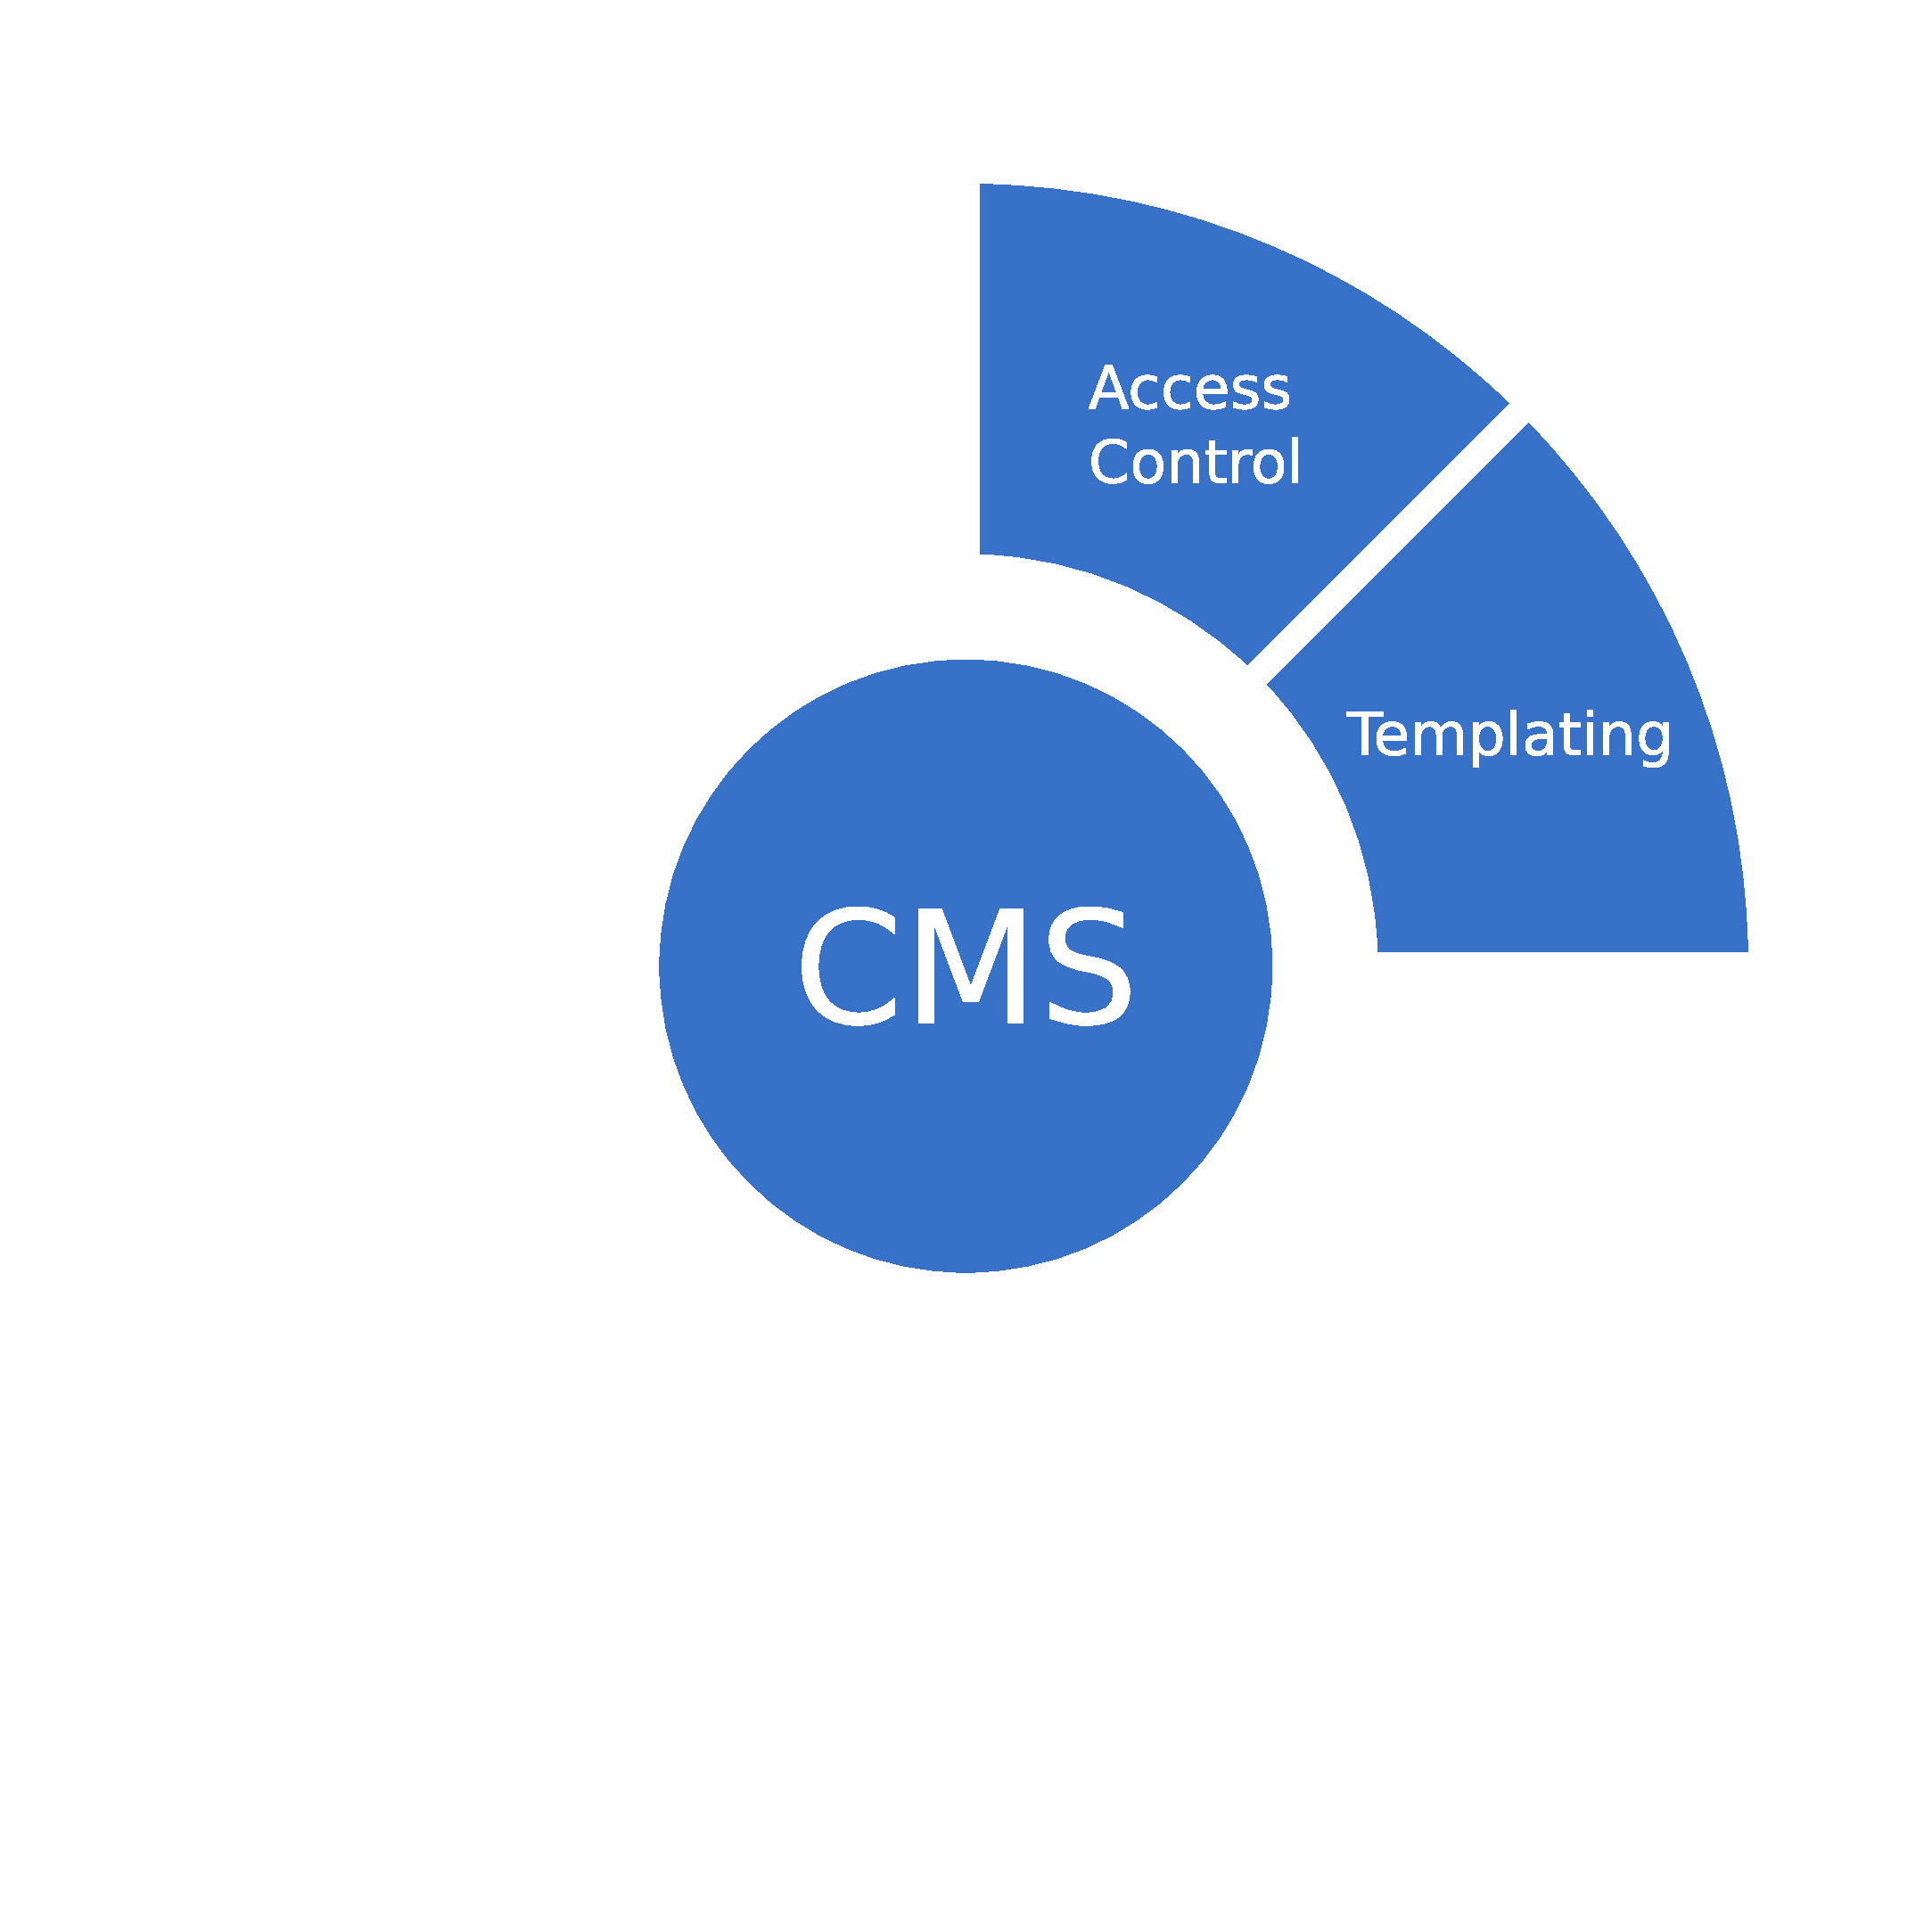
\includegraphics[height=\textheight]{cms-templating.pdf}}
\frame{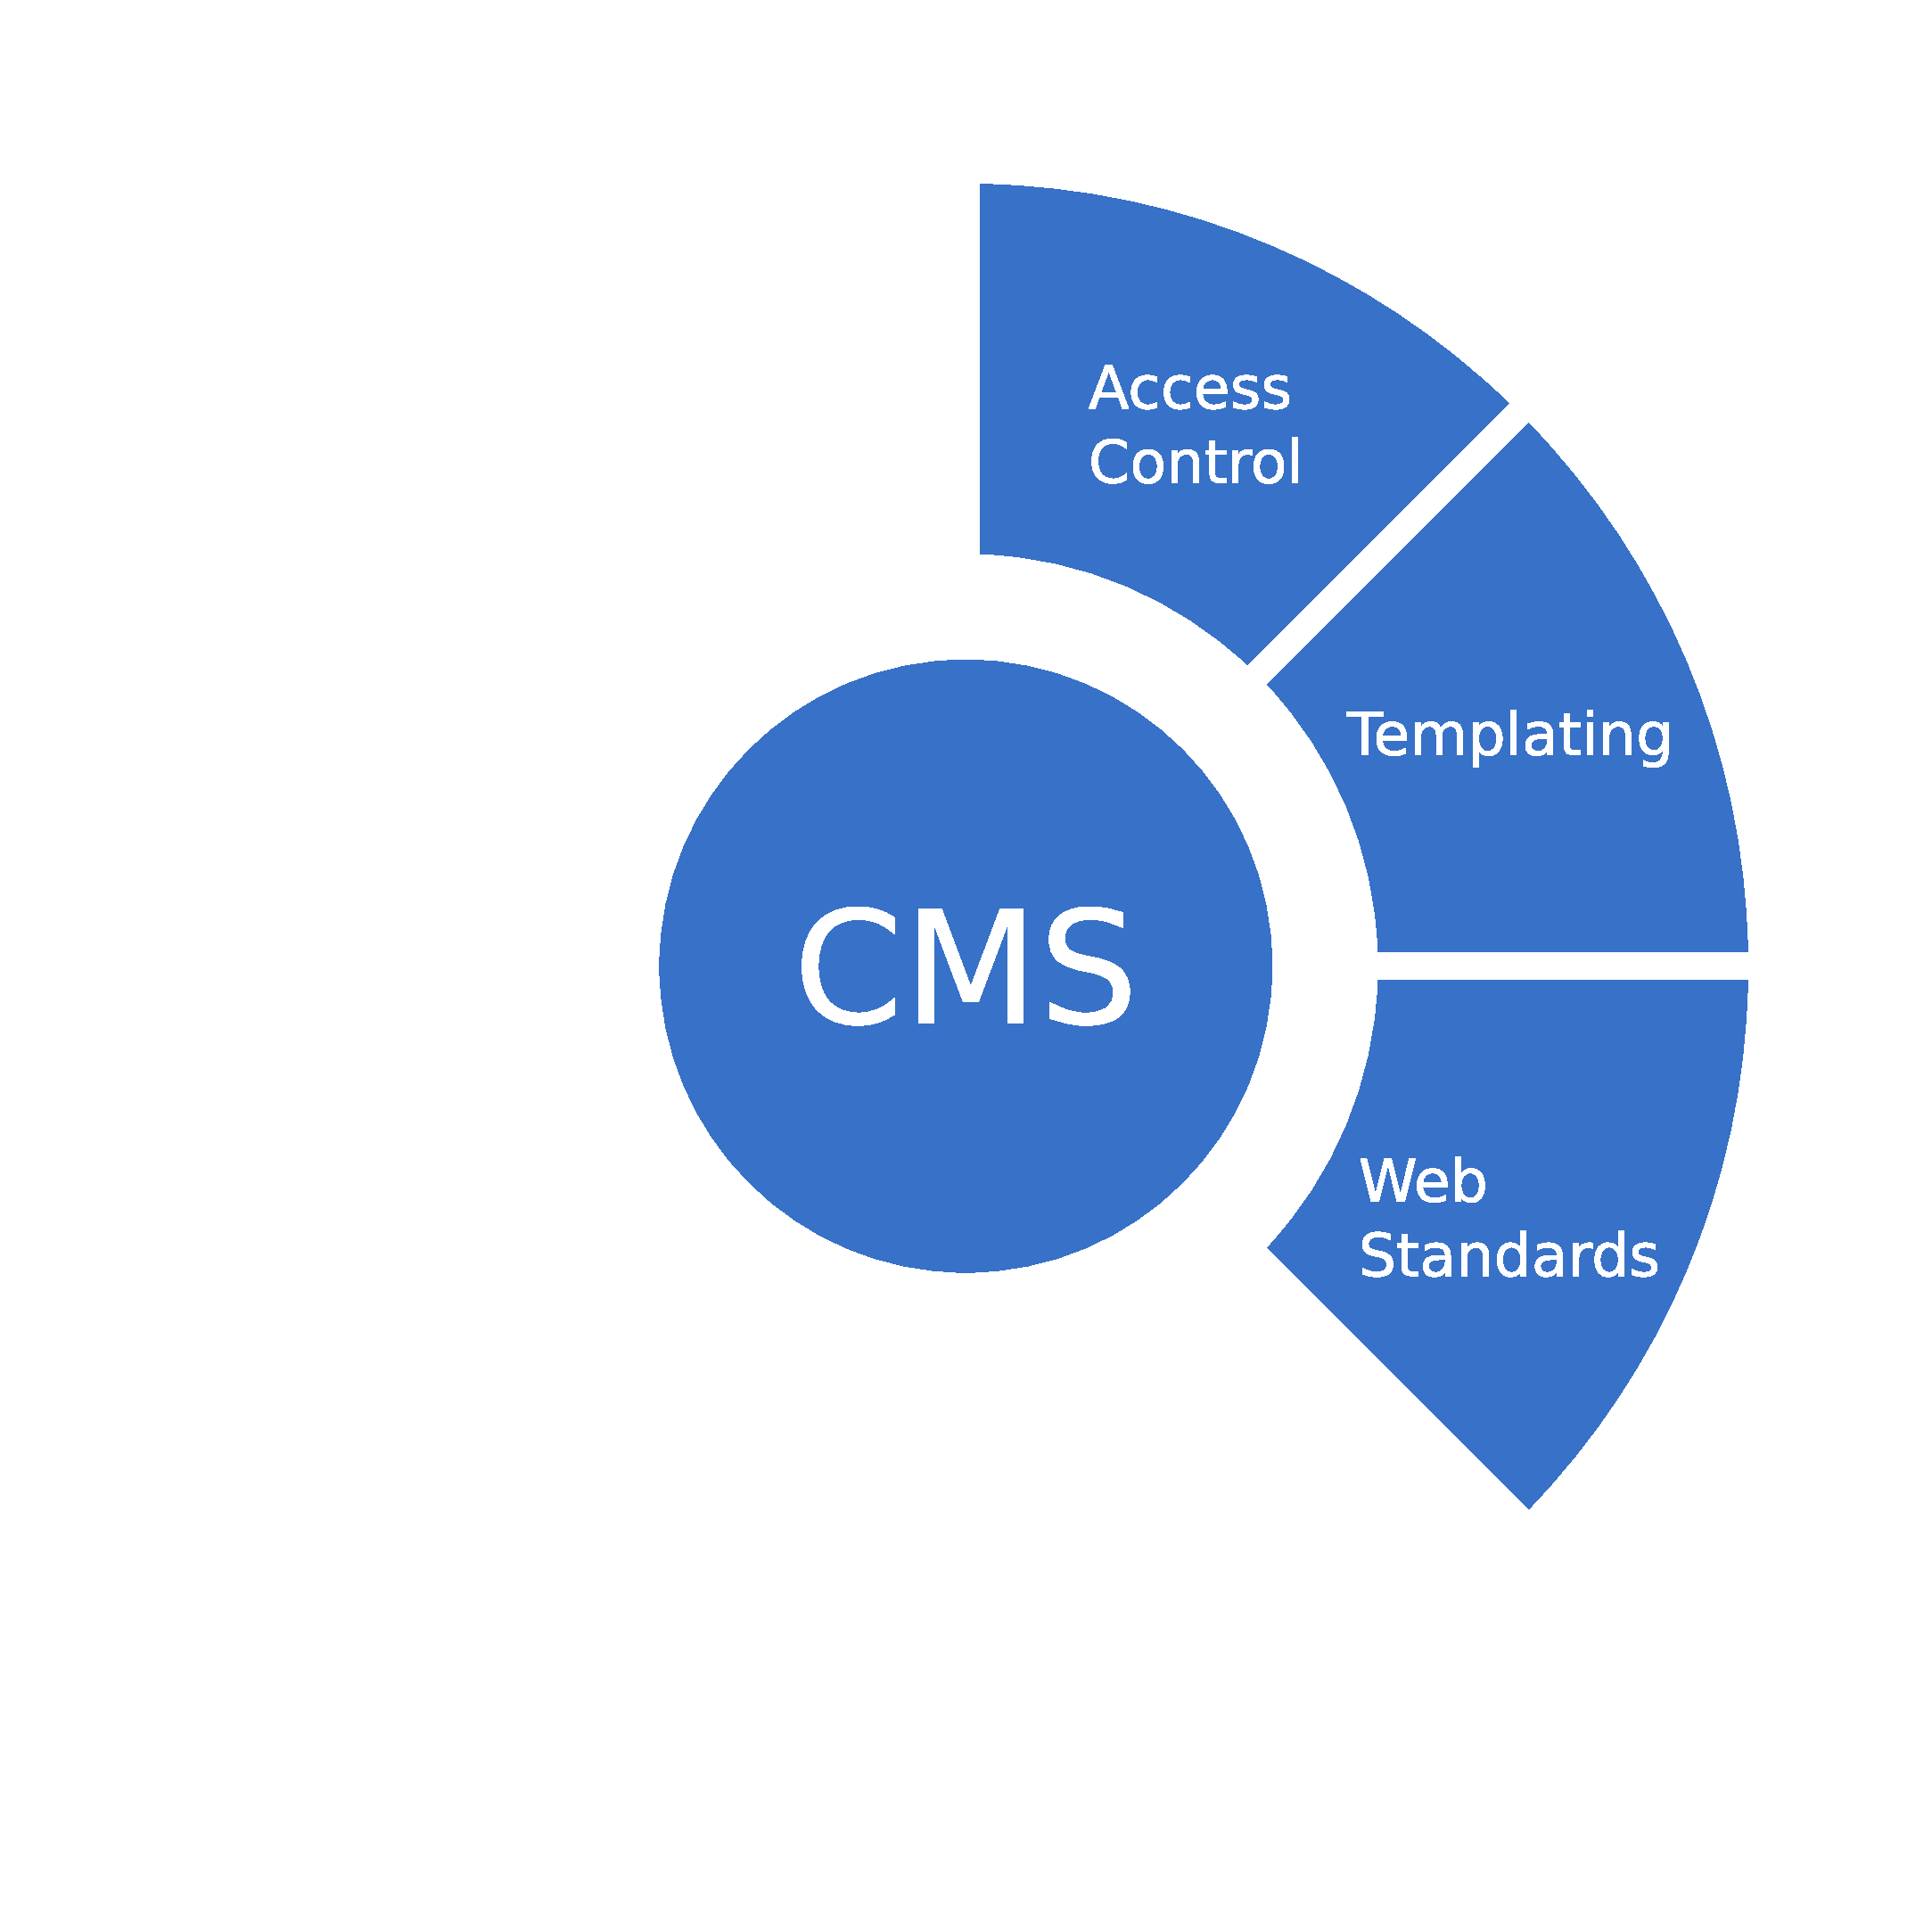
\includegraphics[height=\textheight]{cms-web-standards.pdf}}
\frame{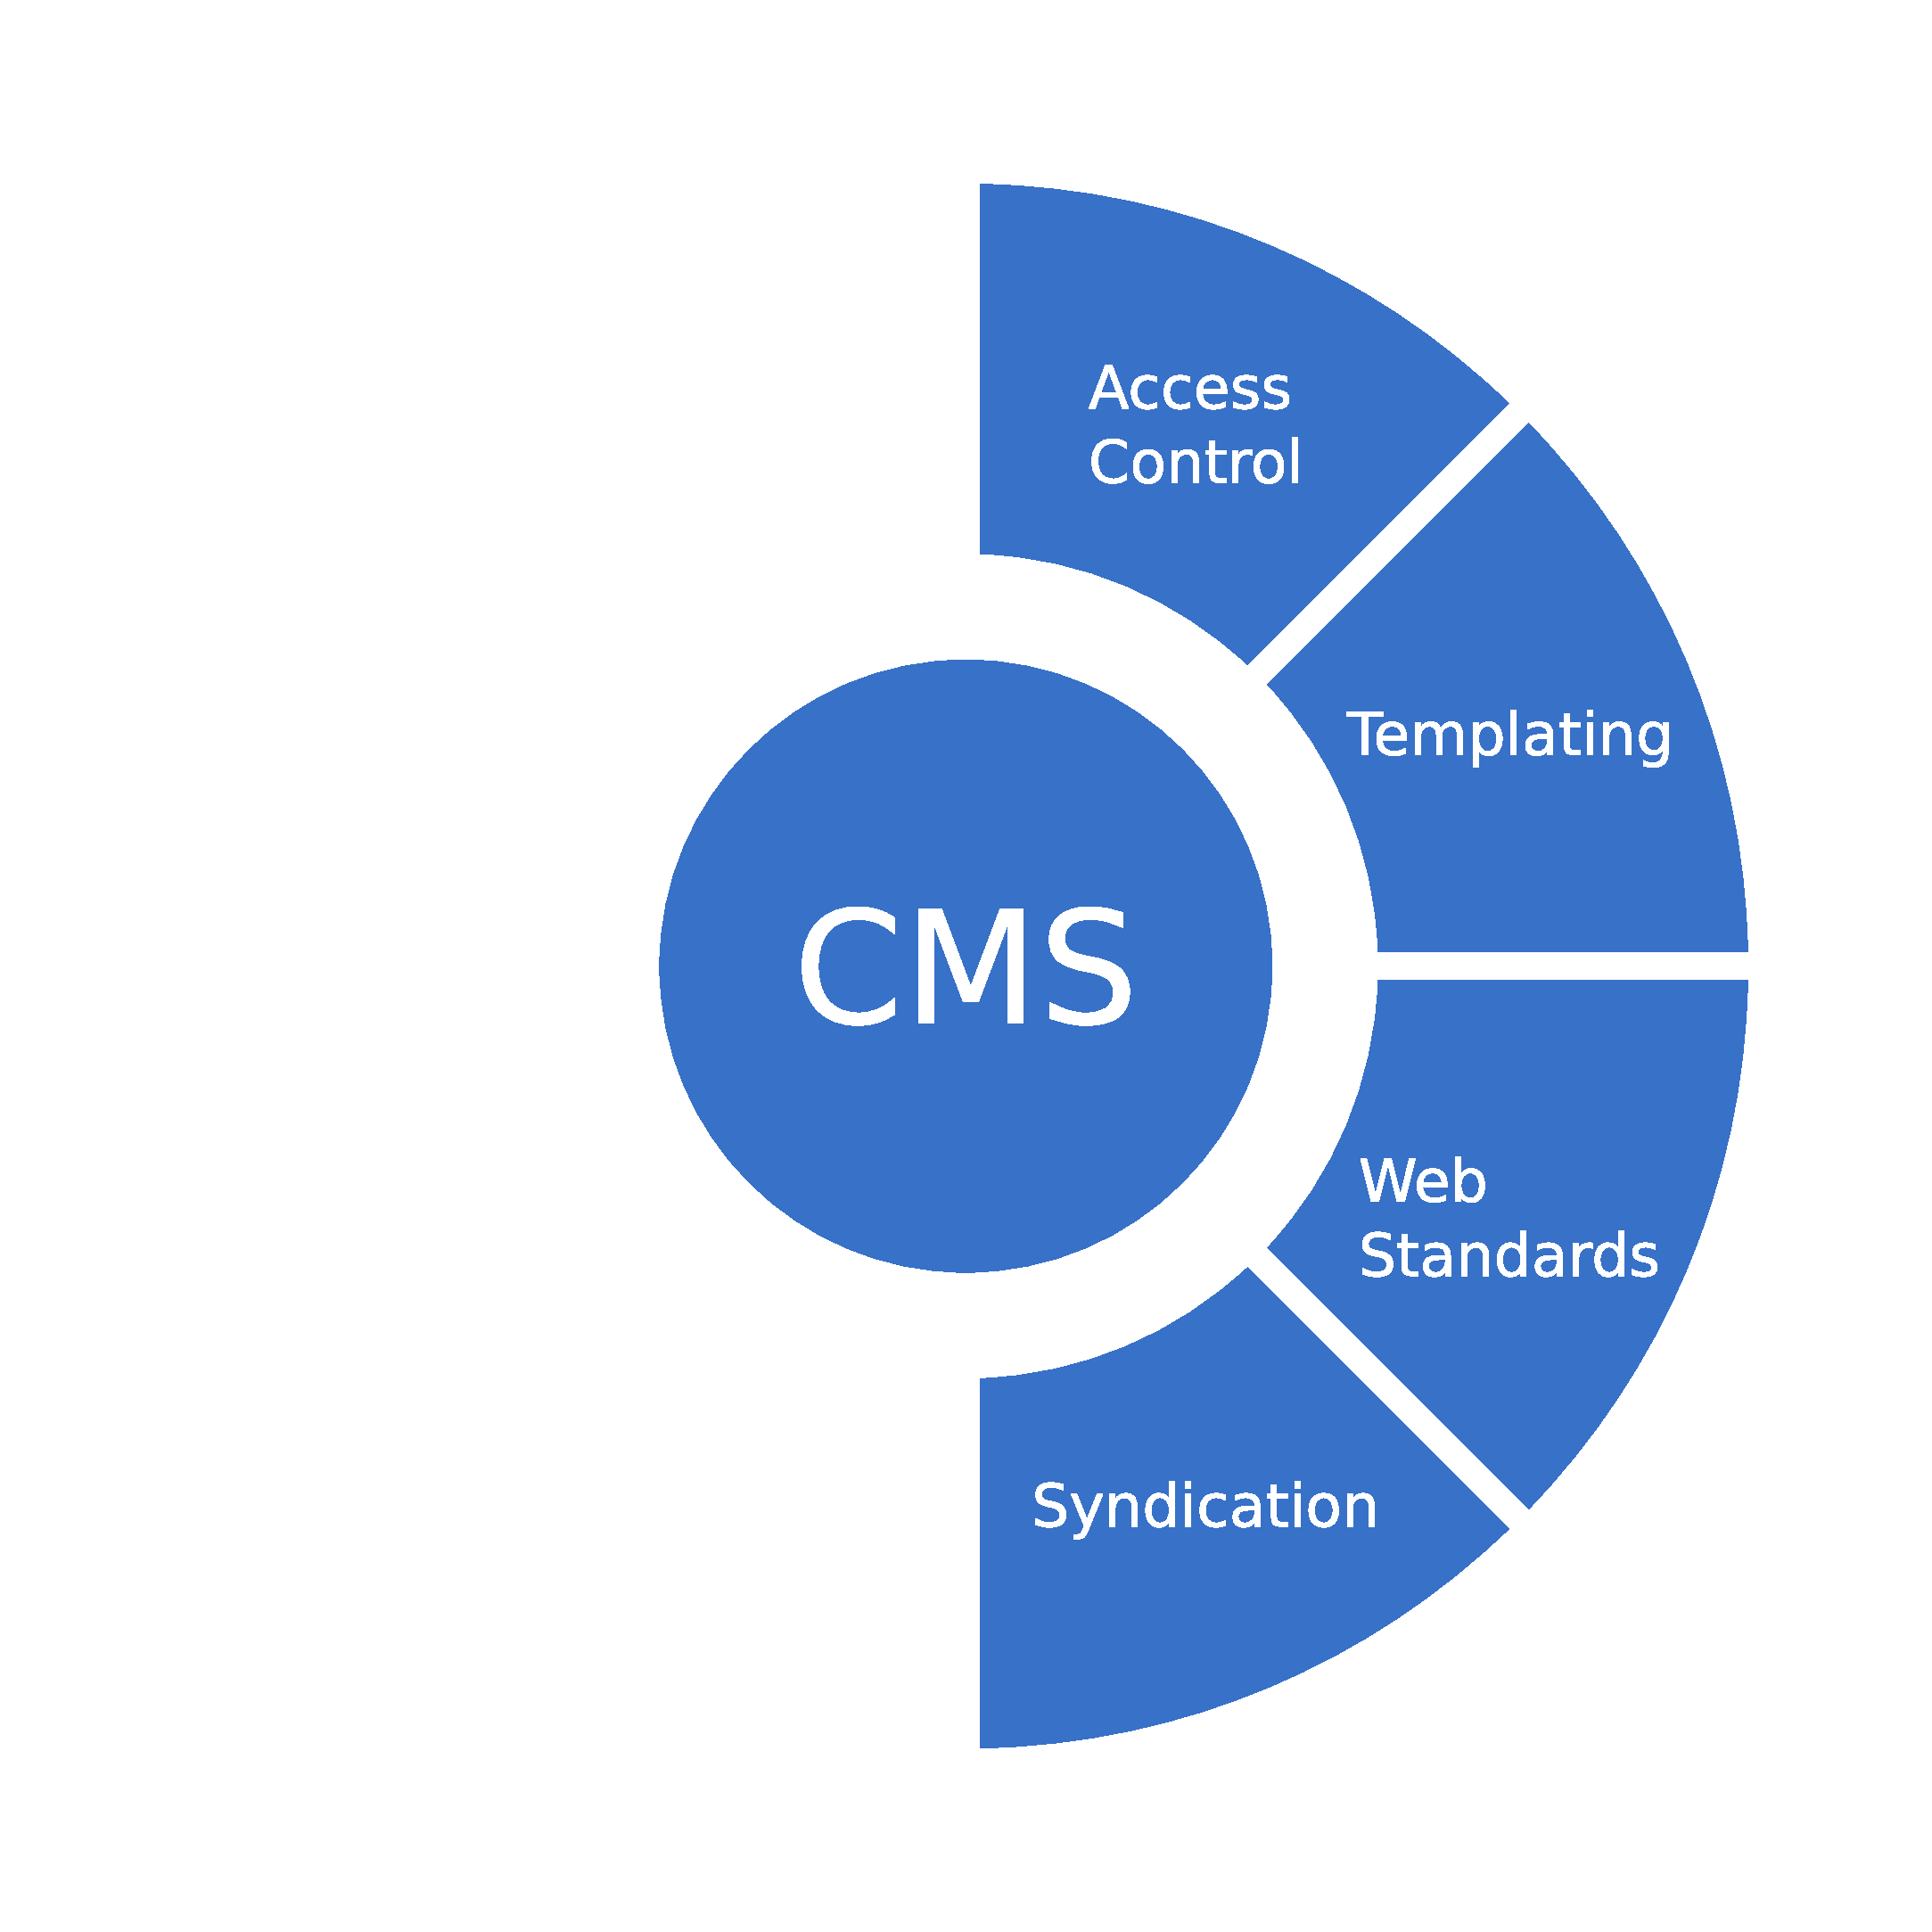
\includegraphics[height=\textheight]{cms-syndication.pdf}}
\frame{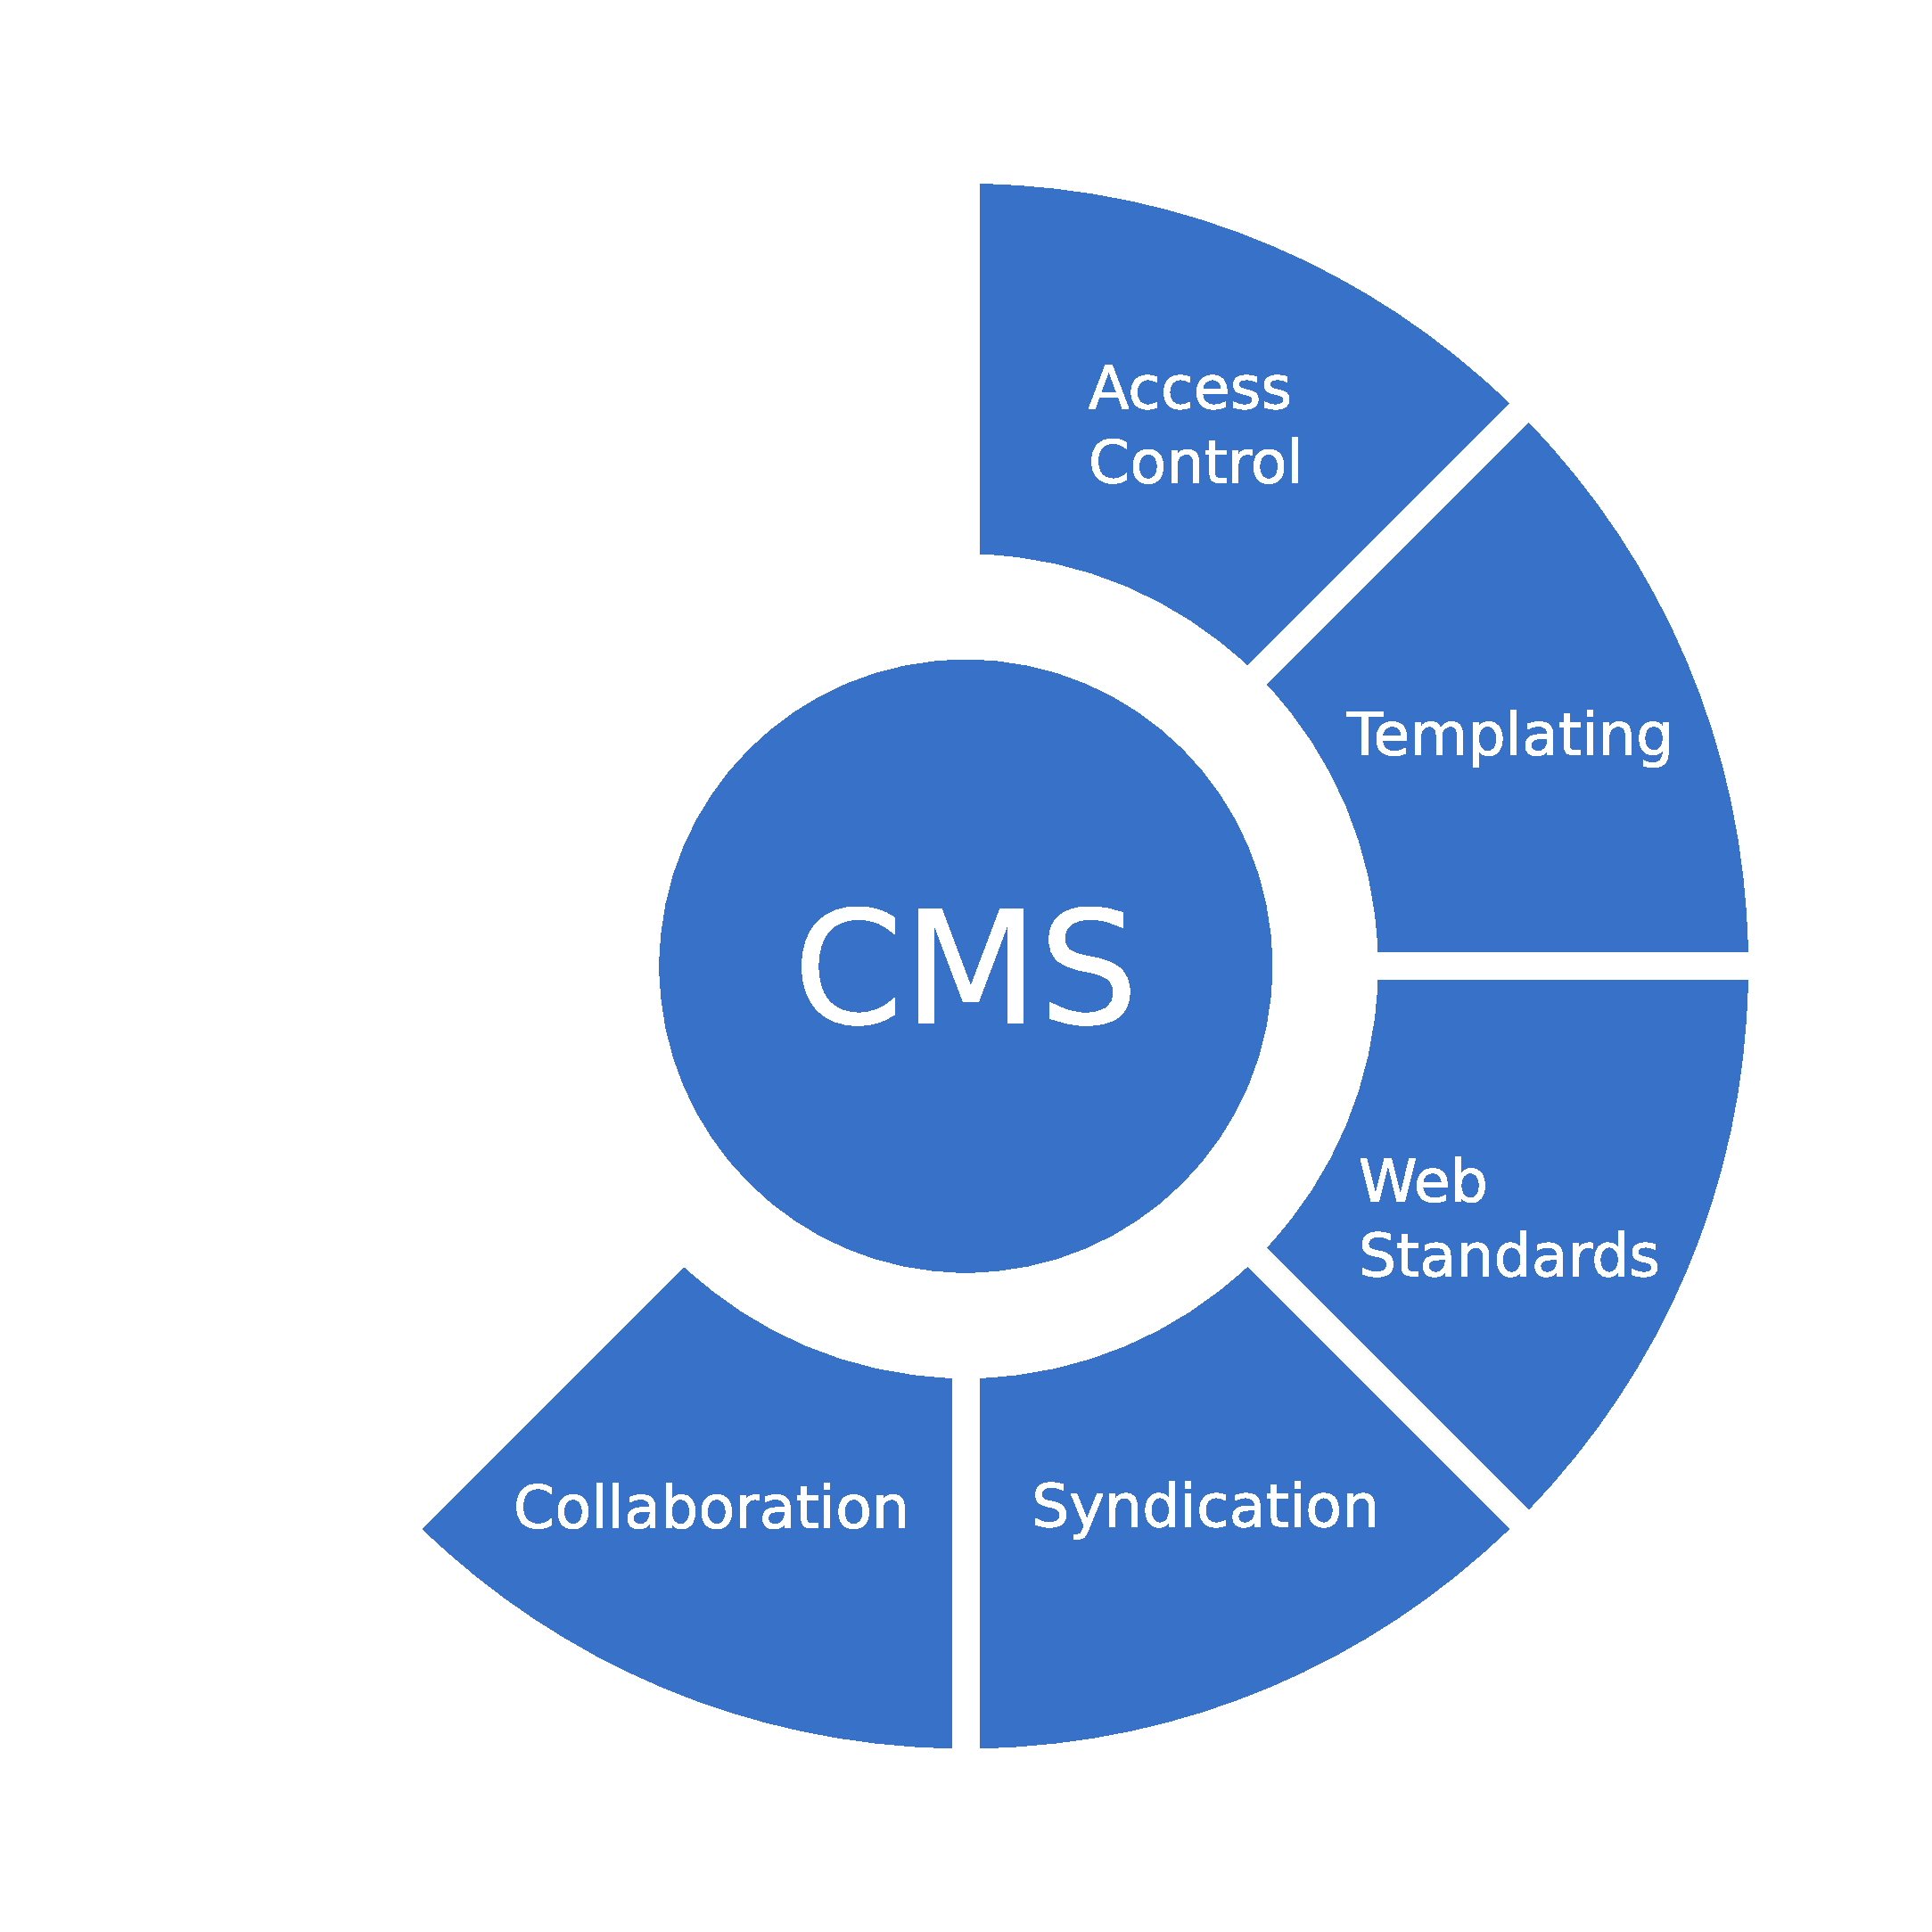
\includegraphics[height=\textheight]{cms-collaboration.pdf}}
\frame{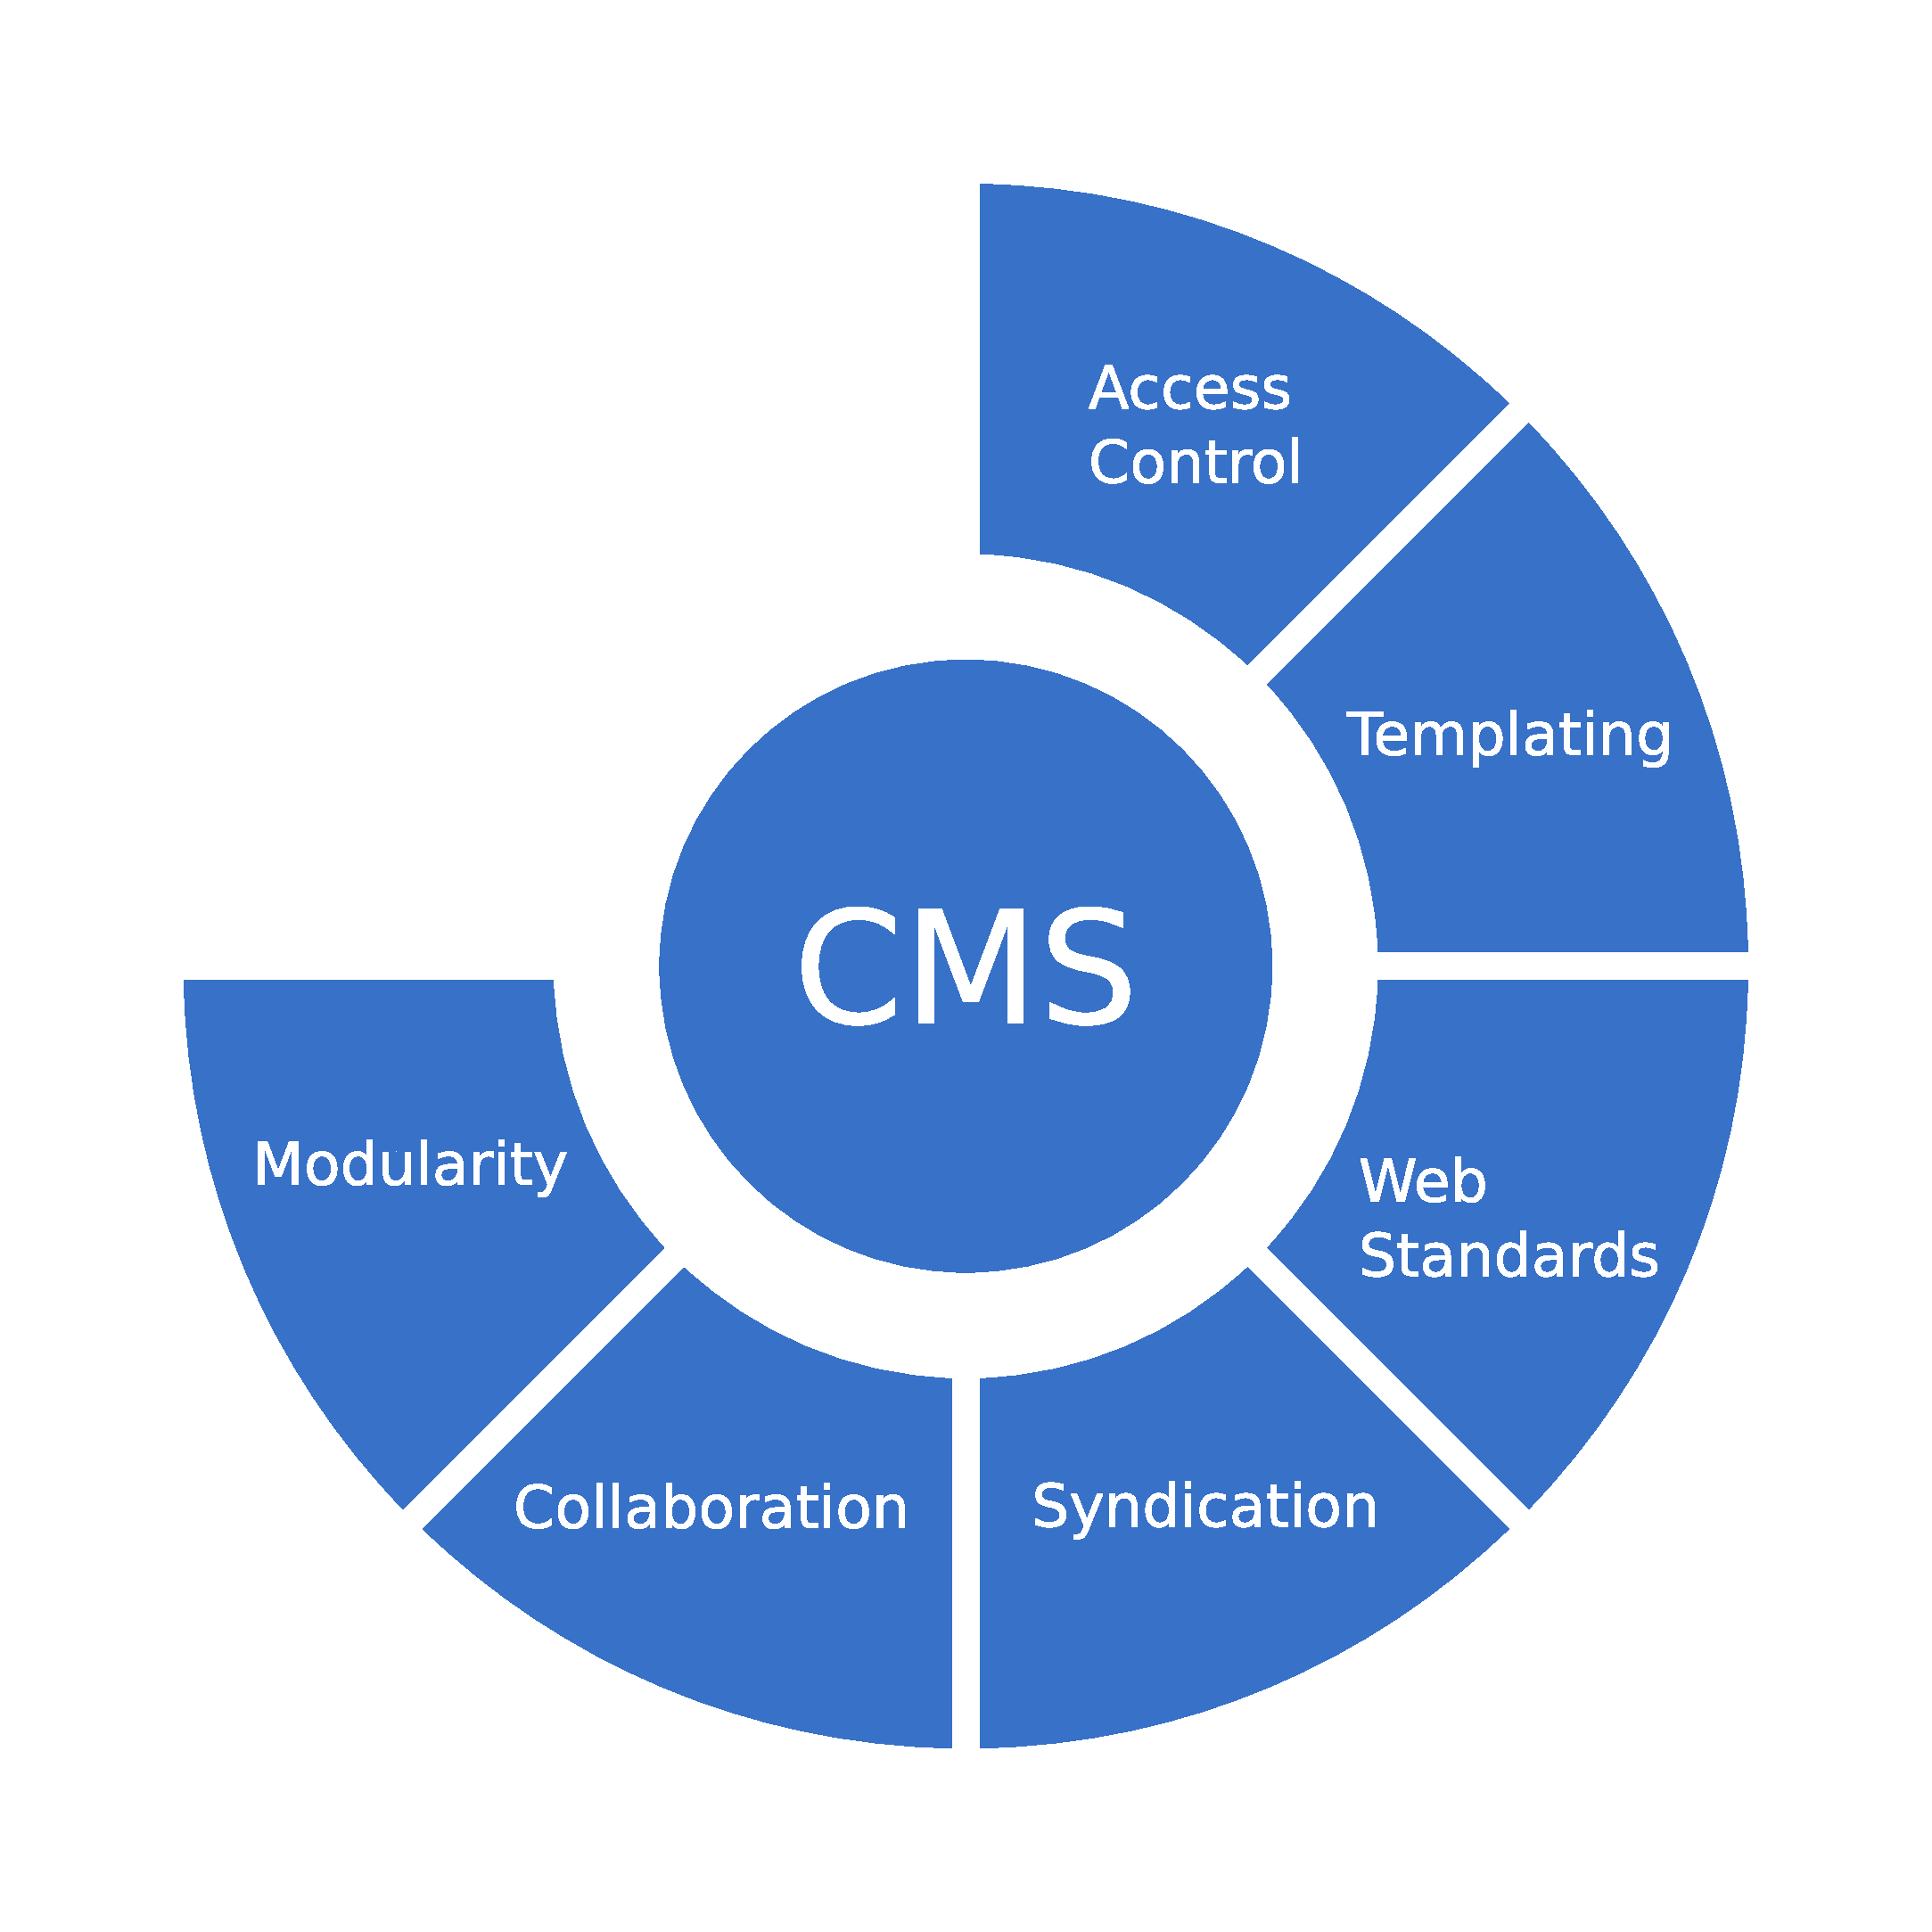
\includegraphics[height=\textheight]{cms-modularity.pdf}}
\frame{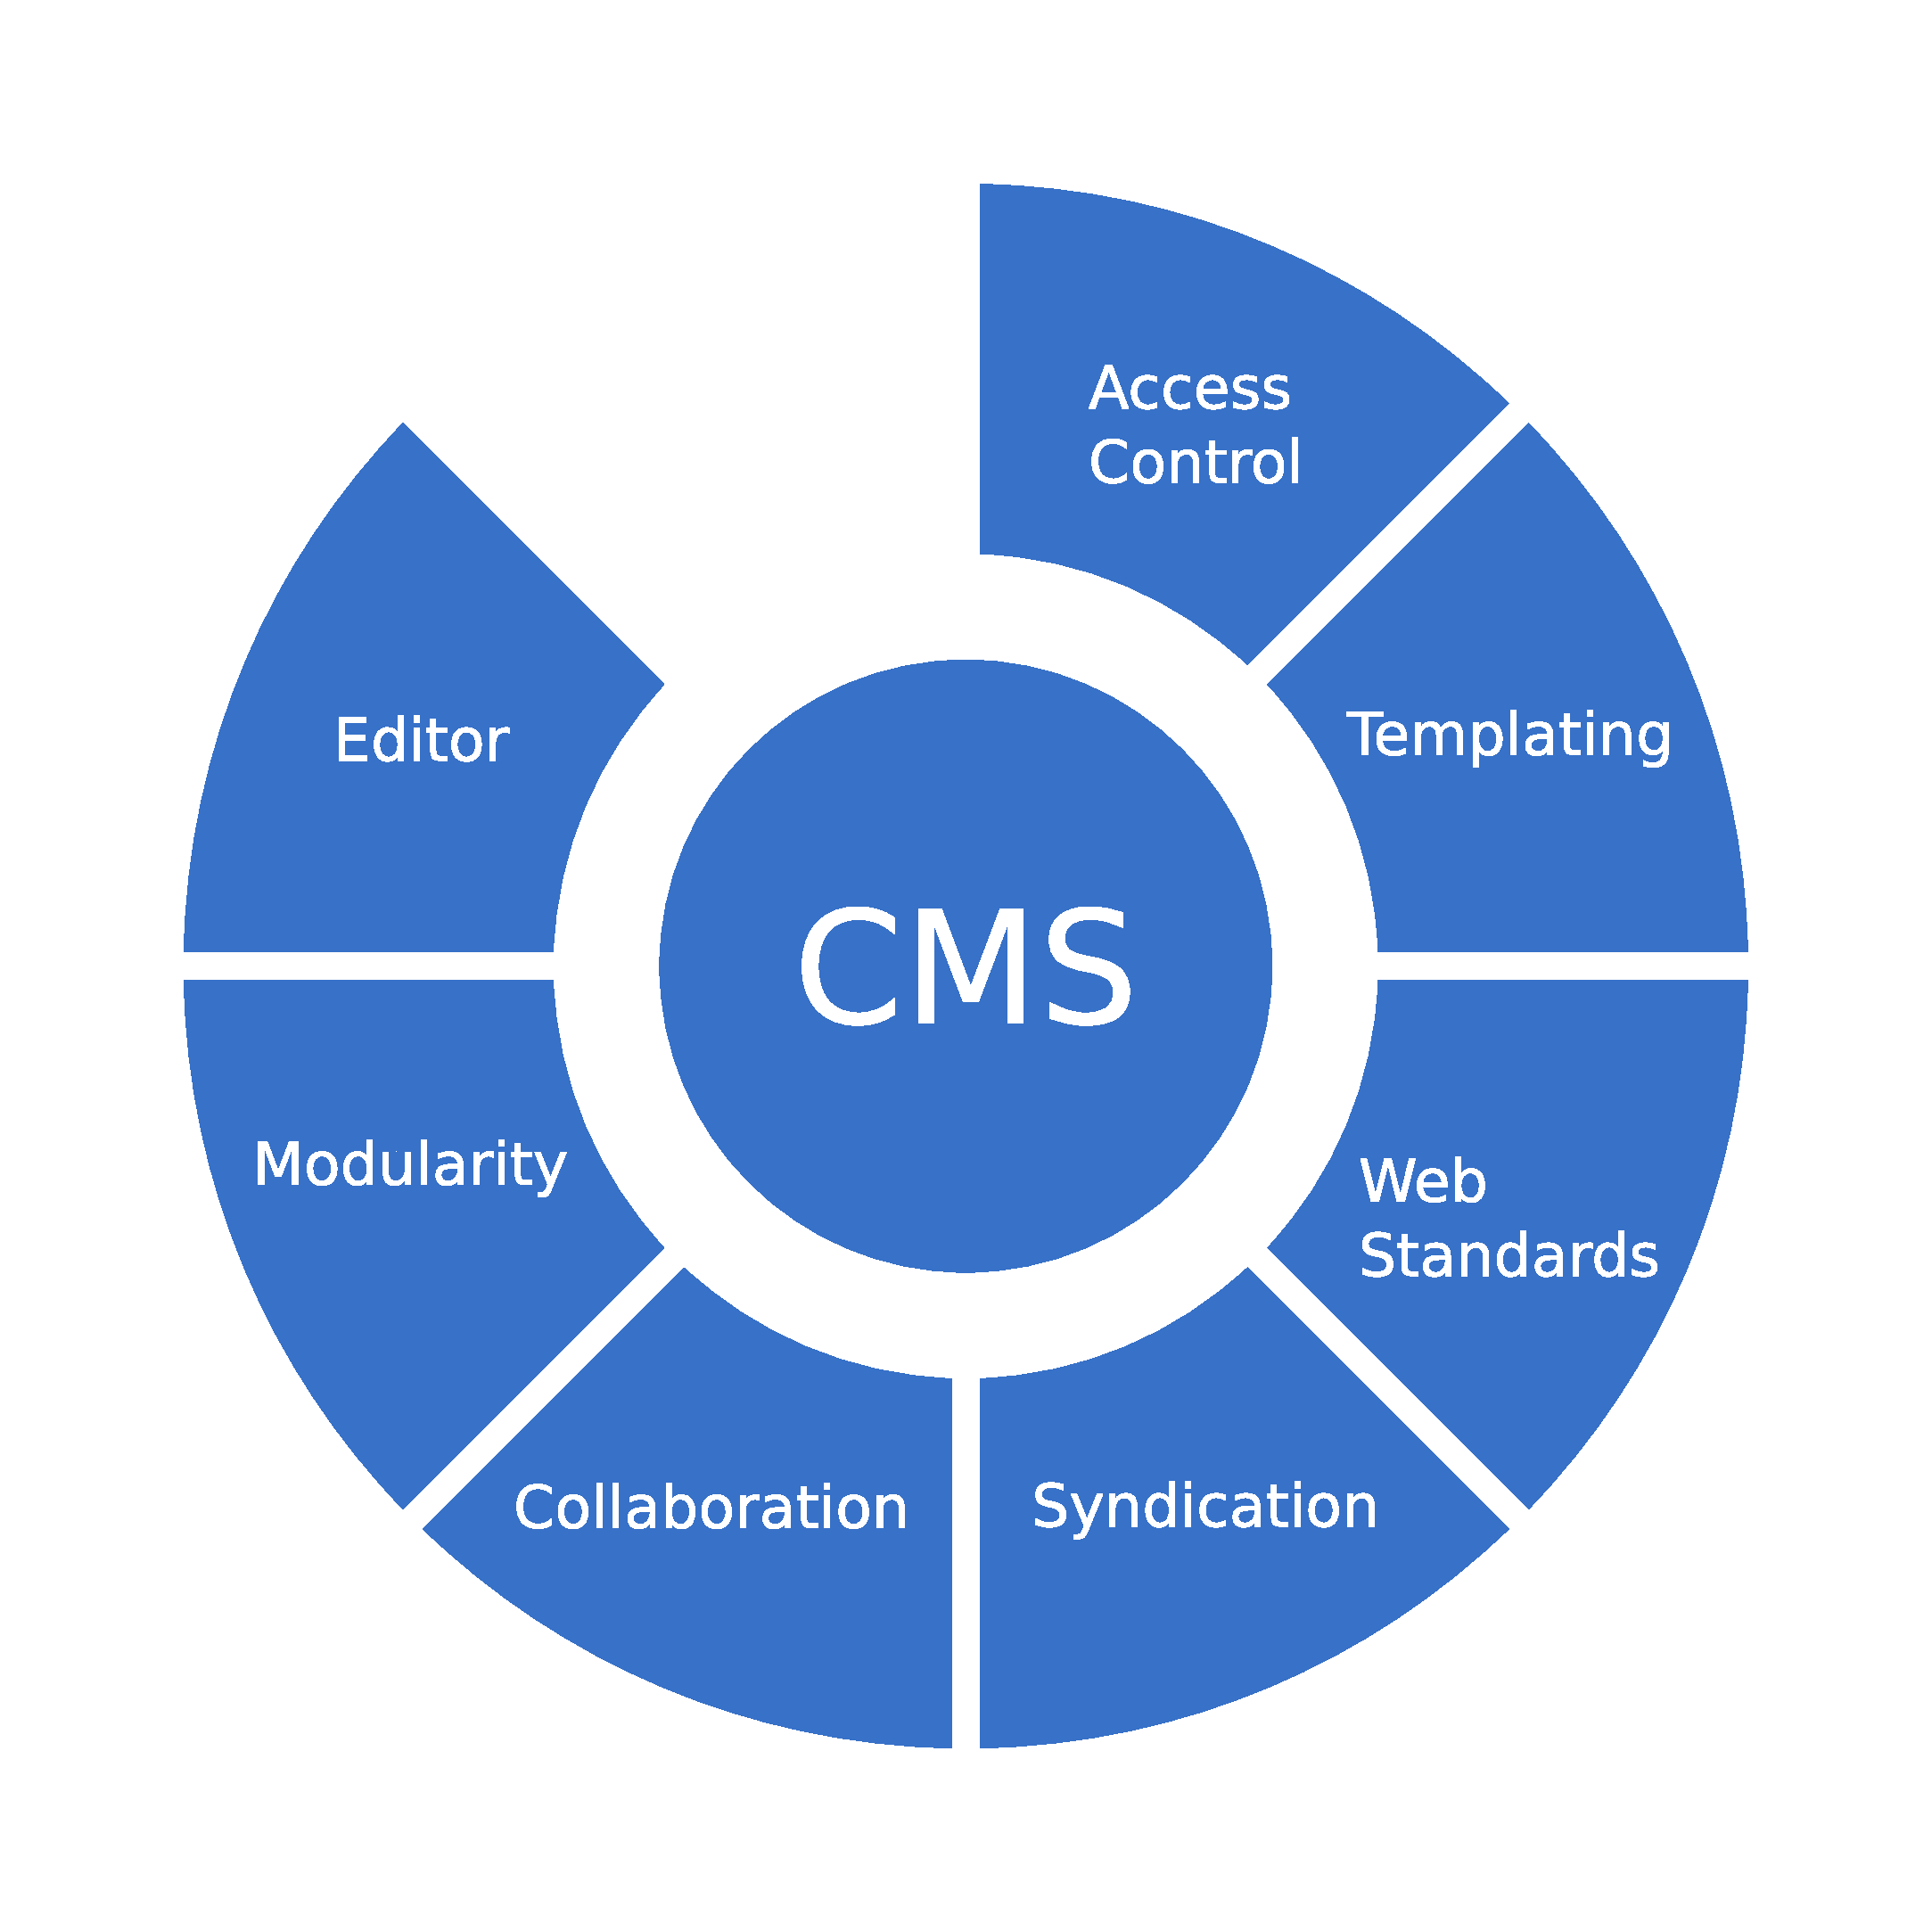
\includegraphics[height=\textheight]{cms-editor.pdf}}
\frame{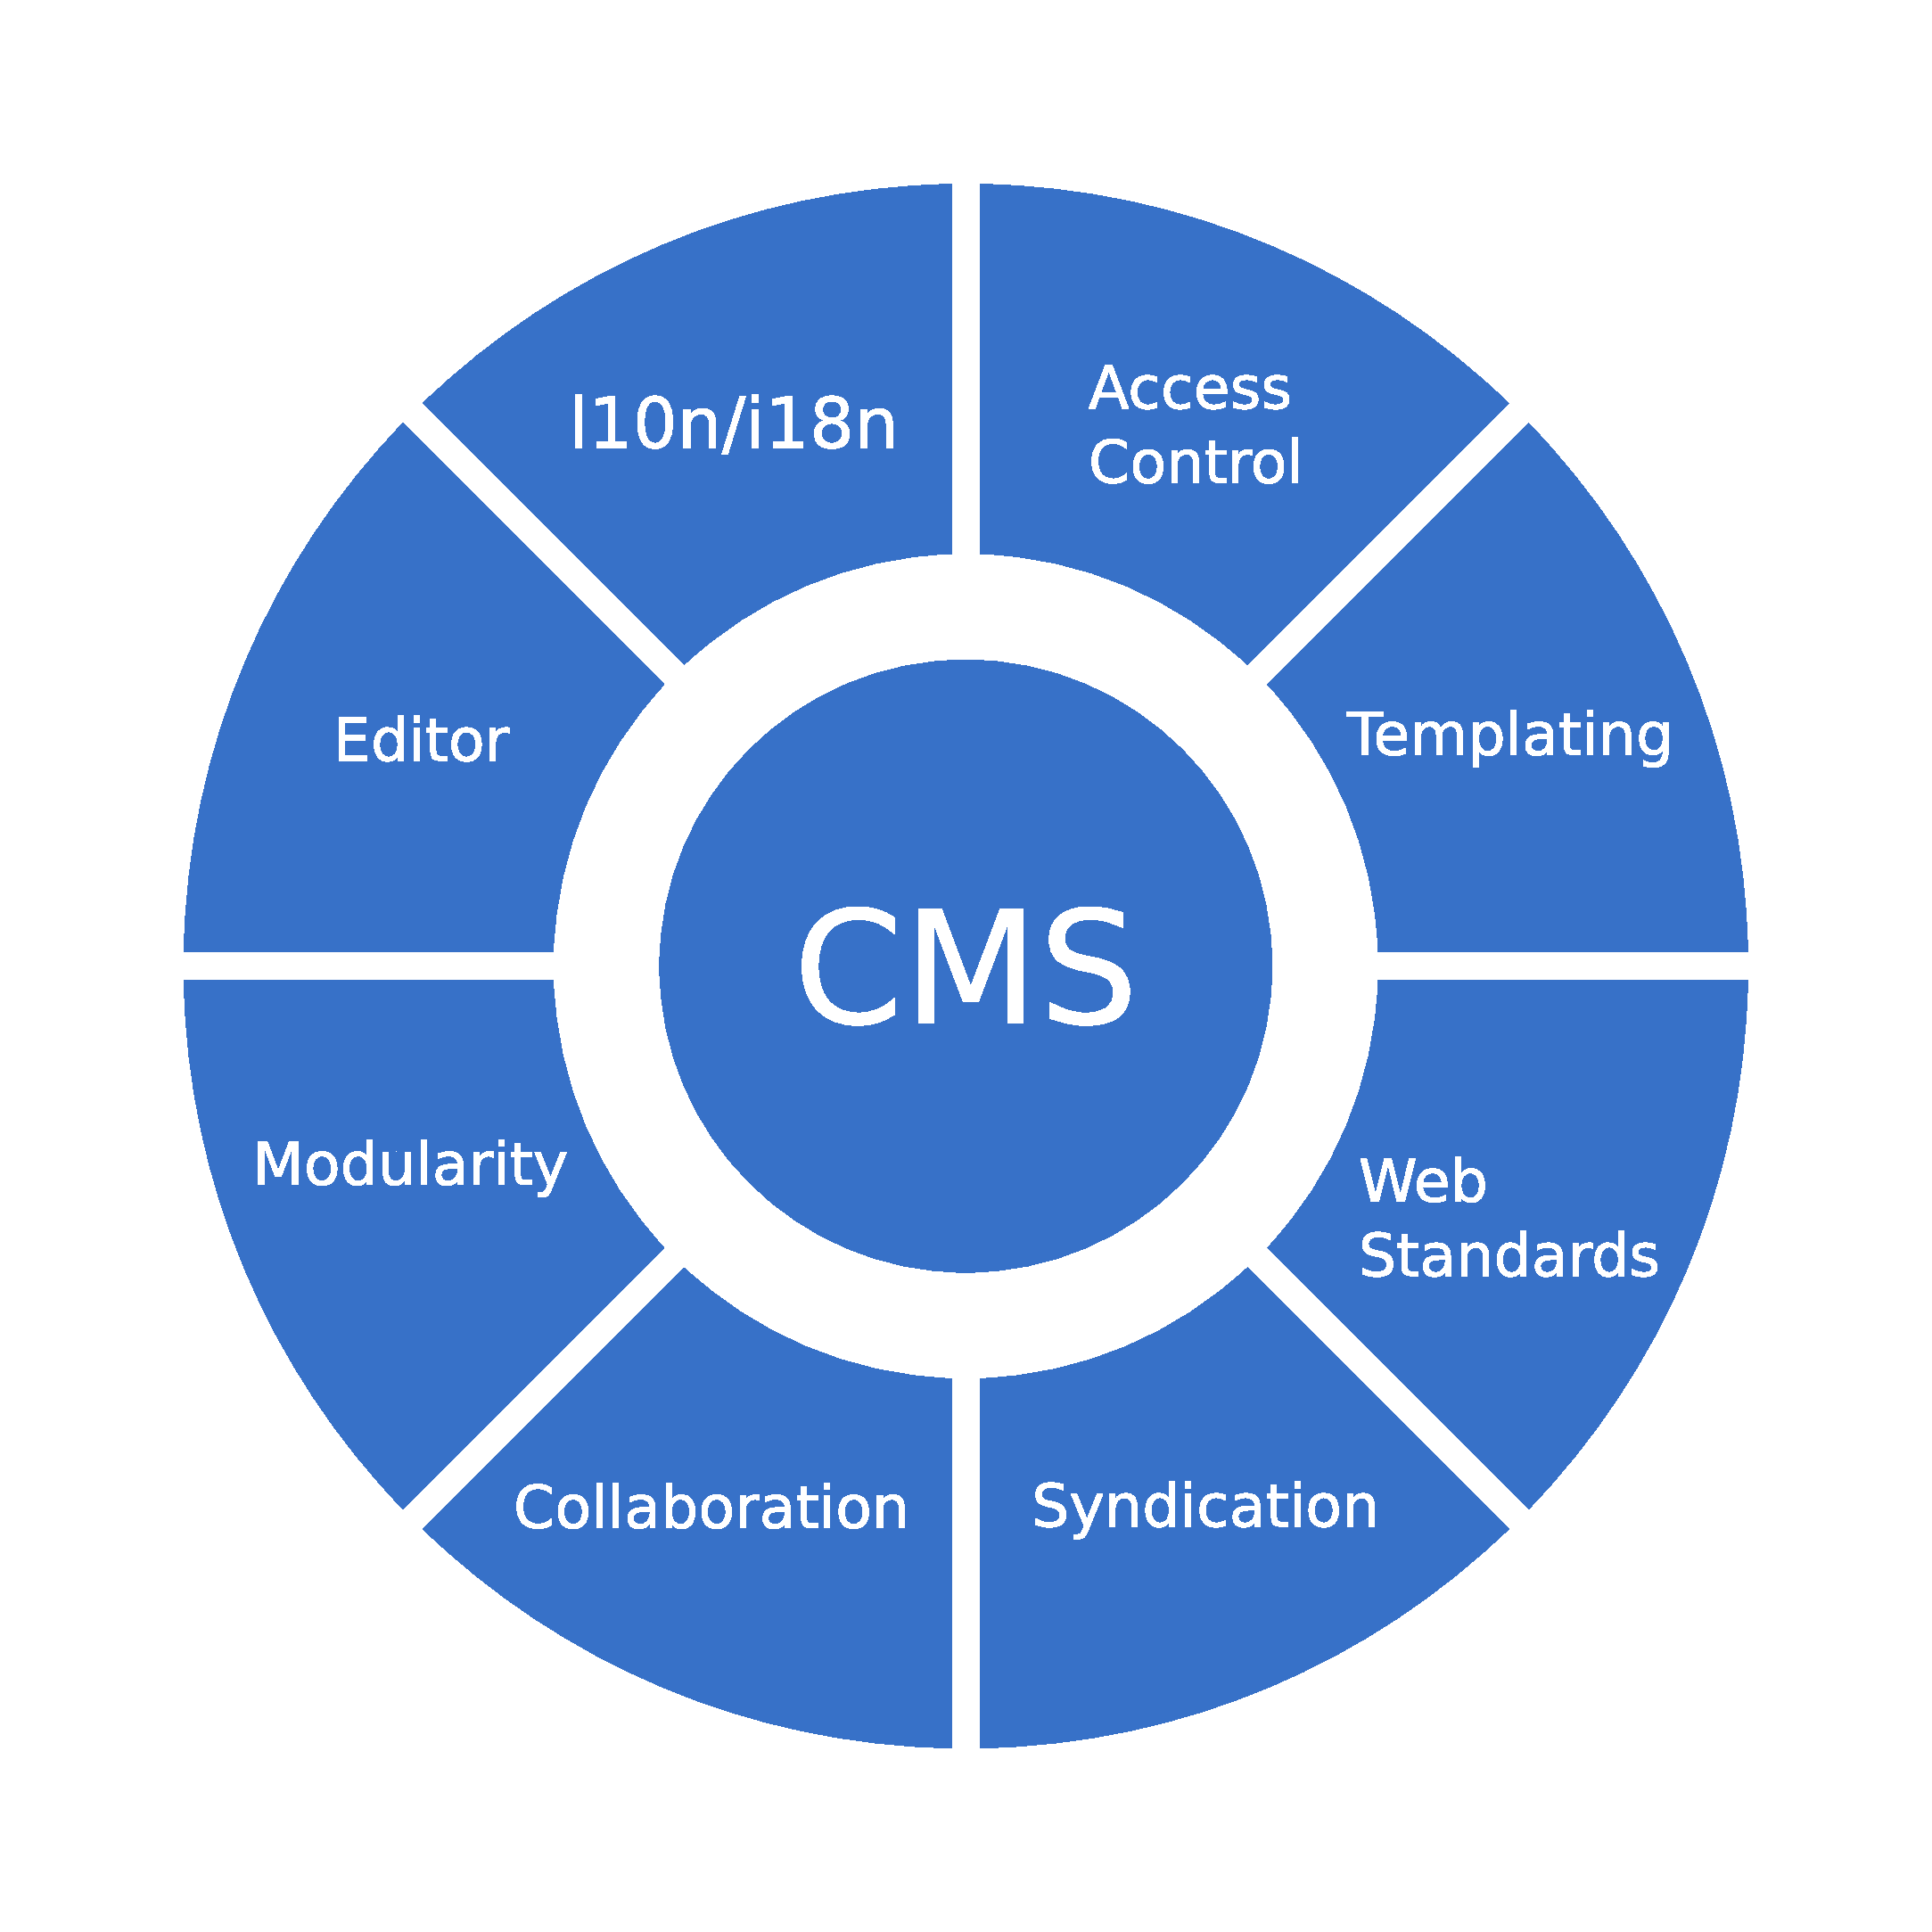
\includegraphics[height=\textheight]{cms-l10n-i18n.pdf}}

\frame{
\includegraphics[width=\textwidth]{example-cms.pdf}}

\section{About Plone}

\frame{
\includegraphics[width=\textwidth]{plone.pdf}}
\frame{
\includegraphics[width=\textwidth]{python.pdf}}
\begin{frame}
  \begin{center}
    
\includegraphics[height=0.5\textheight]{zope.pdf}
  \end{center}
\end{frame}

\section{Easy Startup and Configuration}
\begin{frame}
  
\includegraphics[width=\textwidth]{platforms.pdf} \pause
  \begin{center}
    No dependencies(UnifiedInstaller)
  \end{center}
\end{frame}

\begin{frame}
  \begin{center}
    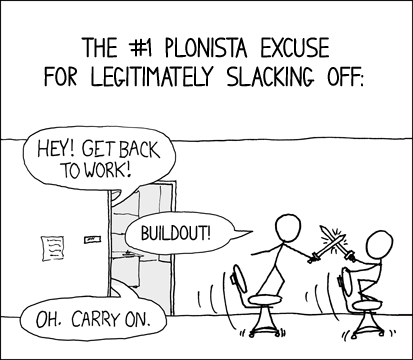
\includegraphics[height=0.7\textheight]{xkcd-buildout.png}
  \end{center}
\end{frame}

\section{I10n/l18n}
\begin{frame}
  \begin{center}
    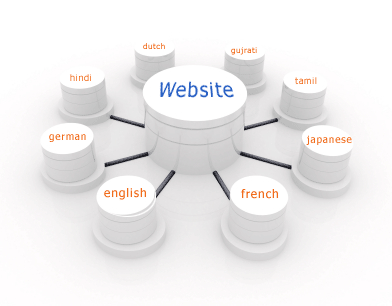
\includegraphics[height=0.7\textheight]{i18n.png}
  \end{center}
\end{frame}

\section{Collective}
\frame{ Open repository at plone collective }
% also mention how awesome it is that you have commit access everywhere
% community built on trust
\frame{number of products available products}

\section{Data Organization}
\frame{hierarchical data organization}
% folderish objects+views have a pic about this

\section{Search}
\frame{First one to have live ajax search, can have RSS on any search}
\frame{contant type: collection}
\frame{in-document searching}

\section{Security}
\begin{frame}{Lies, Damn Lies and Statistics}
  \centering
  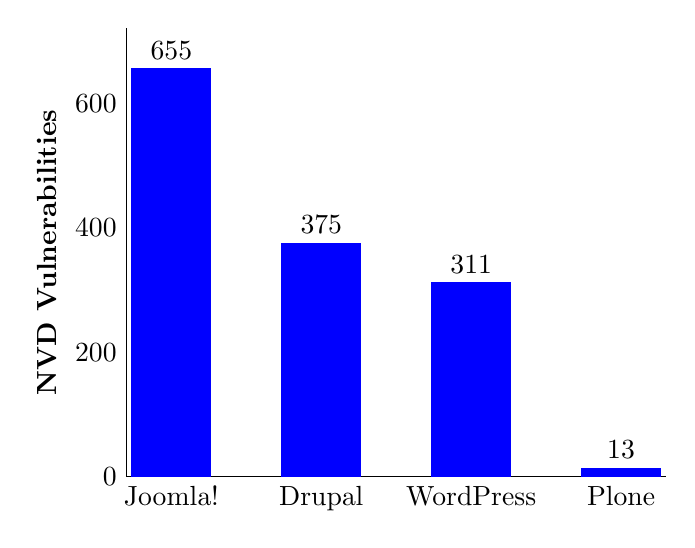
\begin{tikzpicture}
    \begin{axis}
      [ybar, bar width=1cm,
      axis x line*=bottom,
      axis y line*=left,
      nodes near coords,
      legend pos=south east,
      ylabel=\textbf{NVD Vulnerabilities},
      xtick=data,
      % x tick label style={/pgf/number format/1000 sep=},
      xticklabels={Joomla!,Drupal,WordPress,Plone},
      major tick length=0,
      ymin=0
      ]
      \addplot[fill=blue, draw=blue] coordinates
      {(1,655)
        (2,375)
        (3,311)
        (4,13)};
    \end{axis}
  \end{tikzpicture}
\end{frame}

\begin{frame}{Lies, Damn Lies and Statistics}
  \centering
  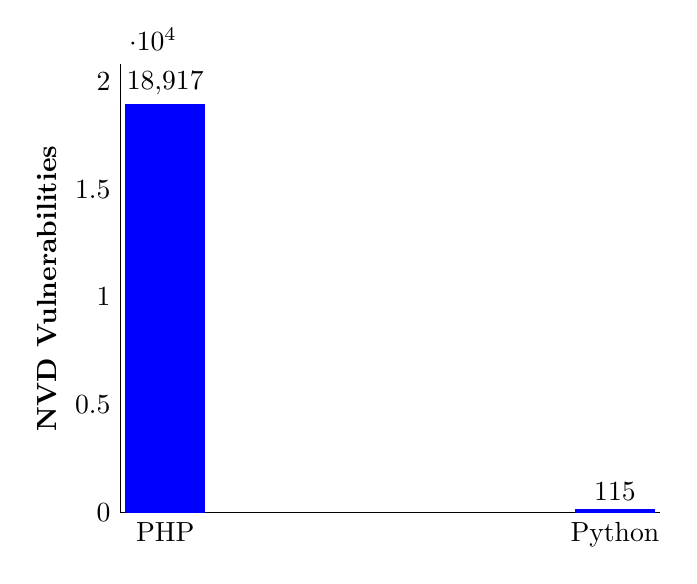
\begin{tikzpicture}
    \begin{axis}
      [ybar, bar width=1cm,
      axis x line*=bottom,
      axis y line*=left,
      nodes near coords,
      legend pos=south east,
      ylabel=\textbf{NVD Vulnerabilities},
      xtick=data,
      %x tick label style={/pgf/number format/1000 sep=0pt},
      xticklabels={PHP,Python},
      major tick length=0,
      ymin=0
      ]
      \addplot[fill=blue, draw=blue] coordinates
      {(1,18917)
        (2,115)};
    \end{axis}
  \end{tikzpicture}
\end{frame}



\frame{unix prototype}
\frame{users->roles->permissions->data(states)}

\section{Authentication}

\frame{PlonePAS}

\section{Bling!}
\begin{frame}
  \begin{itemize}
    \pause \item Theming (XDV, CSS optimization, TAL)
    \pause \item Kupu/TinyMCE
    \pause \item Linkchecker
    \pause \item Fast
    \pause \item Accessibility
    \pause \item Compatible with SQL, Oracle
    \pause \item BLOBs
    \pause \item Flashy Javascript(carousel) Fashy Flash
    \pause \item ZMI
  \end{itemize}
\end{frame}

\section{Community}

\frame{300 core devs, 300+service providers, top 2\% of OSS projects}
\frame{7 anual conferences,sprints, IRC events}
\end{document}
